% ============================================================
% FASE 1
% ============================================================

\section{Fase 1. Evaluación del sistema original}
\label{sec:resultados_fase1}

Se identificaron deficiencias mecánicas en los mecanismos de traslación de los ejes X, Y y Z. La configuración inicial incorporó tubos metálicos para instalaciones eléctricas como elementos de guiado y carros impresos en 3D con rodamientos radiales de bolas (Figura~\ref{fig:fase1_vista_general}).

\begin{figure}[H]
    \centering
    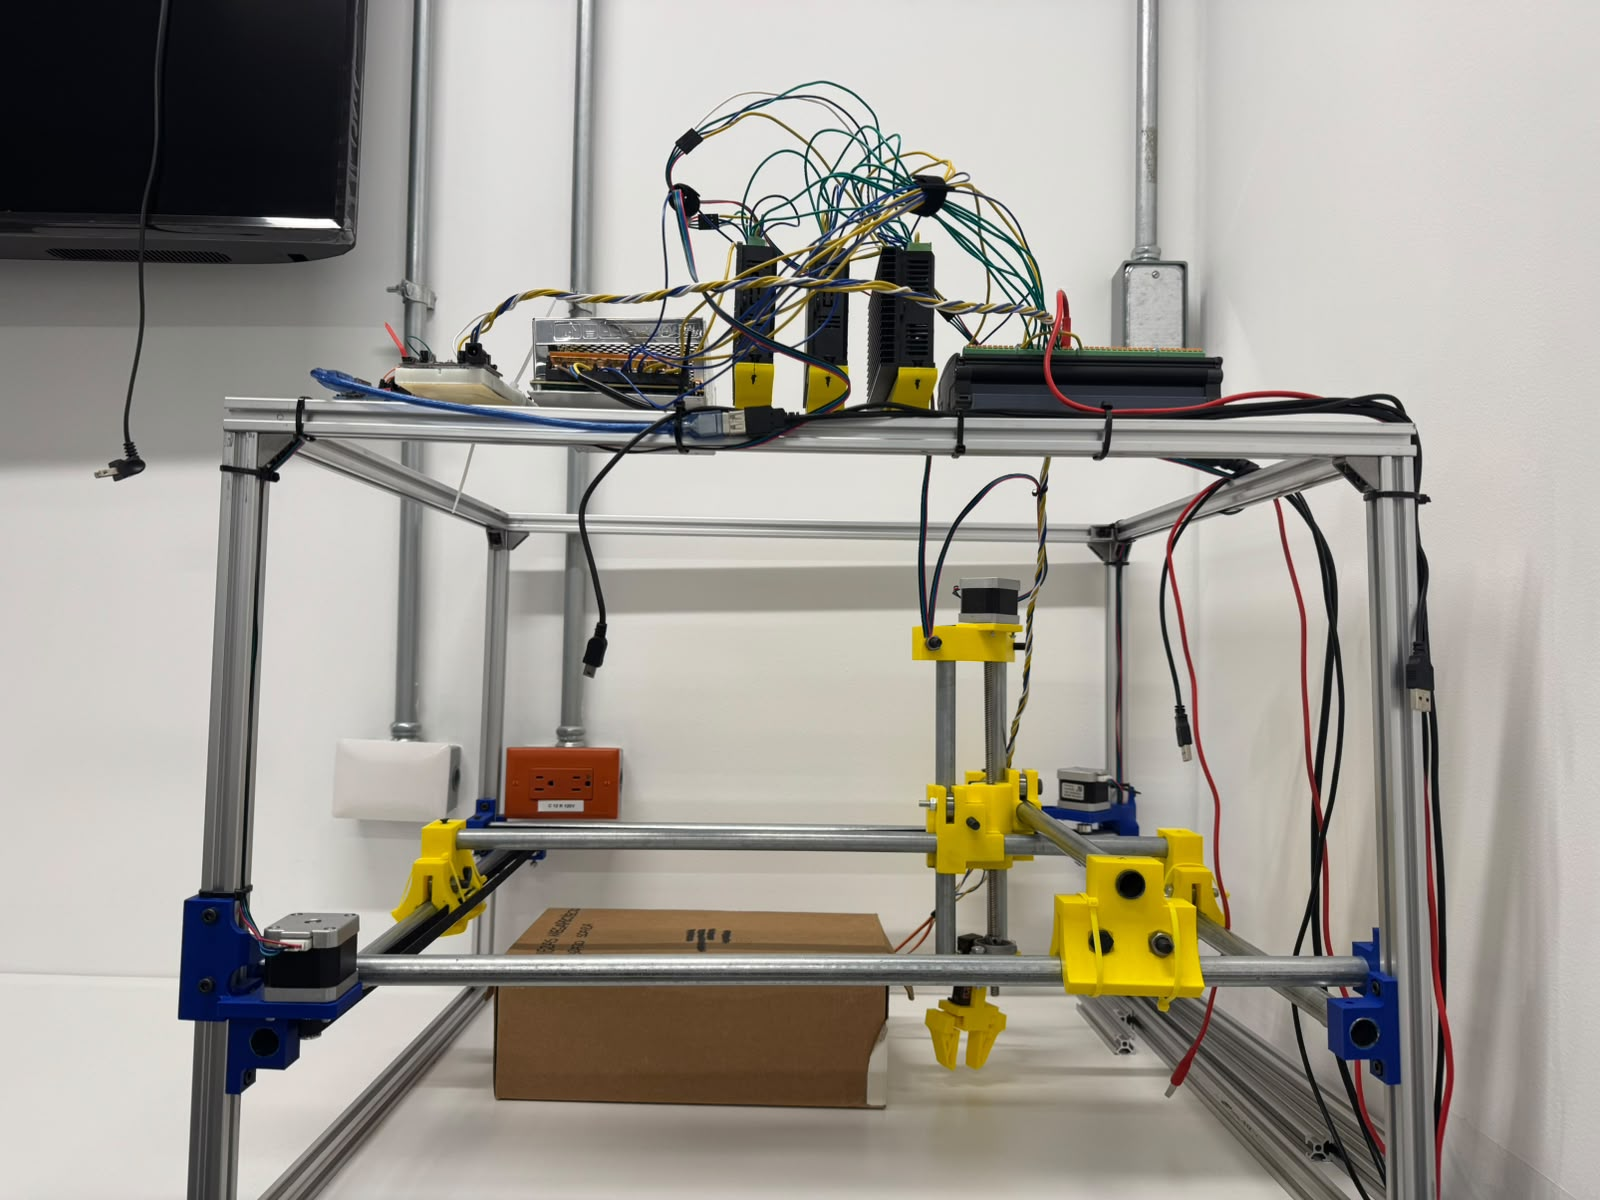
\includegraphics[width=0.75\textwidth,height=6cm,keepaspectratio]
    {Imagenes de Documentacion/F1_1.jpeg}
    \caption{Configuración inicial del brazo robótico cartesiano.}
    \label{fig:fase1_vista_general}
    \par\small Fuente: elaboración propia.
\end{figure}

En los cuatro carros de X y Y se observó resistencia al desplazamiento y falta de alineación con las guías. También se identificó contacto entre las piezas plásticas y los tubos (Figura~\ref{fig:fase1_carro_xy}). Durante el movimiento del pórtico se observó un avance desigual de sus extremos, identificado como \textit{gantry racking}.

\begin{figure}[H]
    \centering
    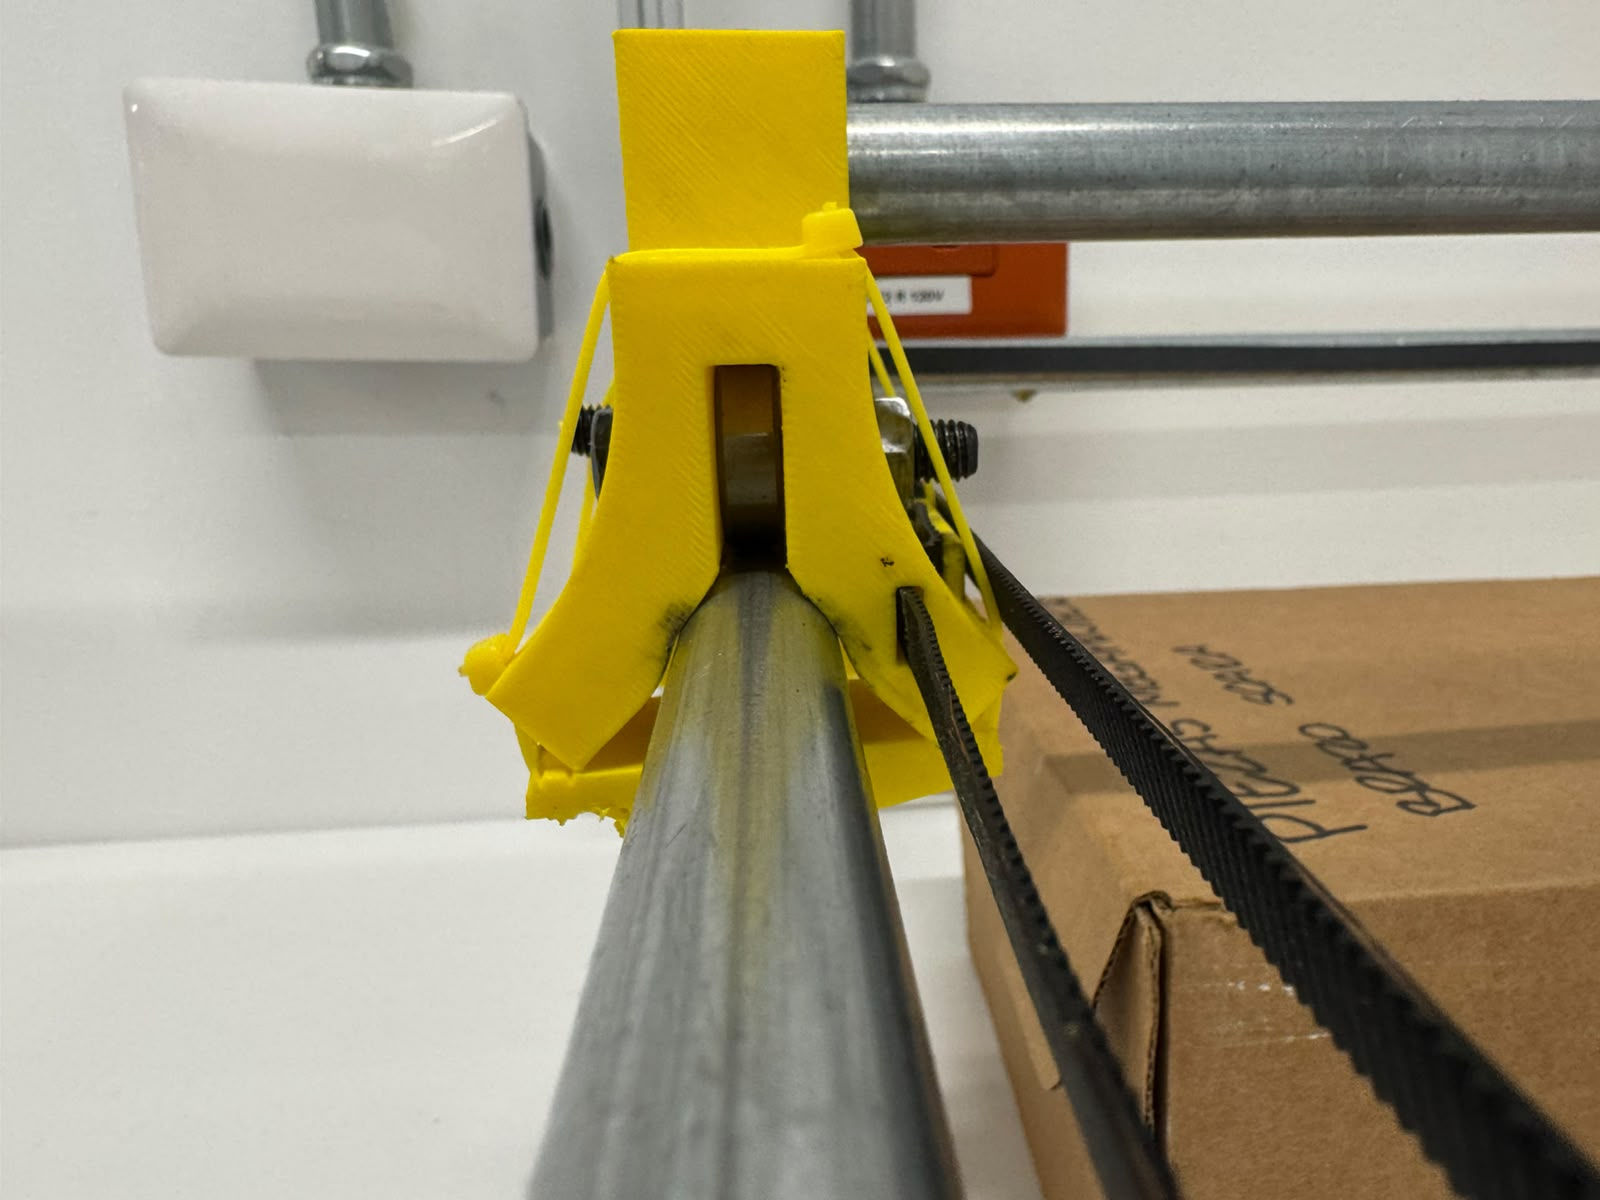
\includegraphics[width=0.65\textwidth,height=5.5cm,keepaspectratio]
    {Imagenes de Documentacion/F1_3.jpeg}
    \caption{Carro y elementos de guiado del sistema original en X y Y.}
    \label{fig:fase1_carro_xy}
    \par\small Fuente: elaboración propia.
\end{figure}

La aplicación de lubricante WD-40 sobre las guías y los carros no eliminó la resistencia al desplazamiento ni el avance desigual del pórtico, lo que indicó que las deficiencias no se debían únicamente a la falta de lubricación.

En Z se observó desalineación del conjunto móvil respecto a la dirección vertical. La disposición del motor, el mecanismo de desplazamiento y la garra se documentó en la Figura~\ref{fig:fase1_eje_z}. Las observaciones de la inspección manual se resumieron en el Cuadro~\ref{tab:fase1_deficiencias}.

\begin{figure}[H]
    \centering
    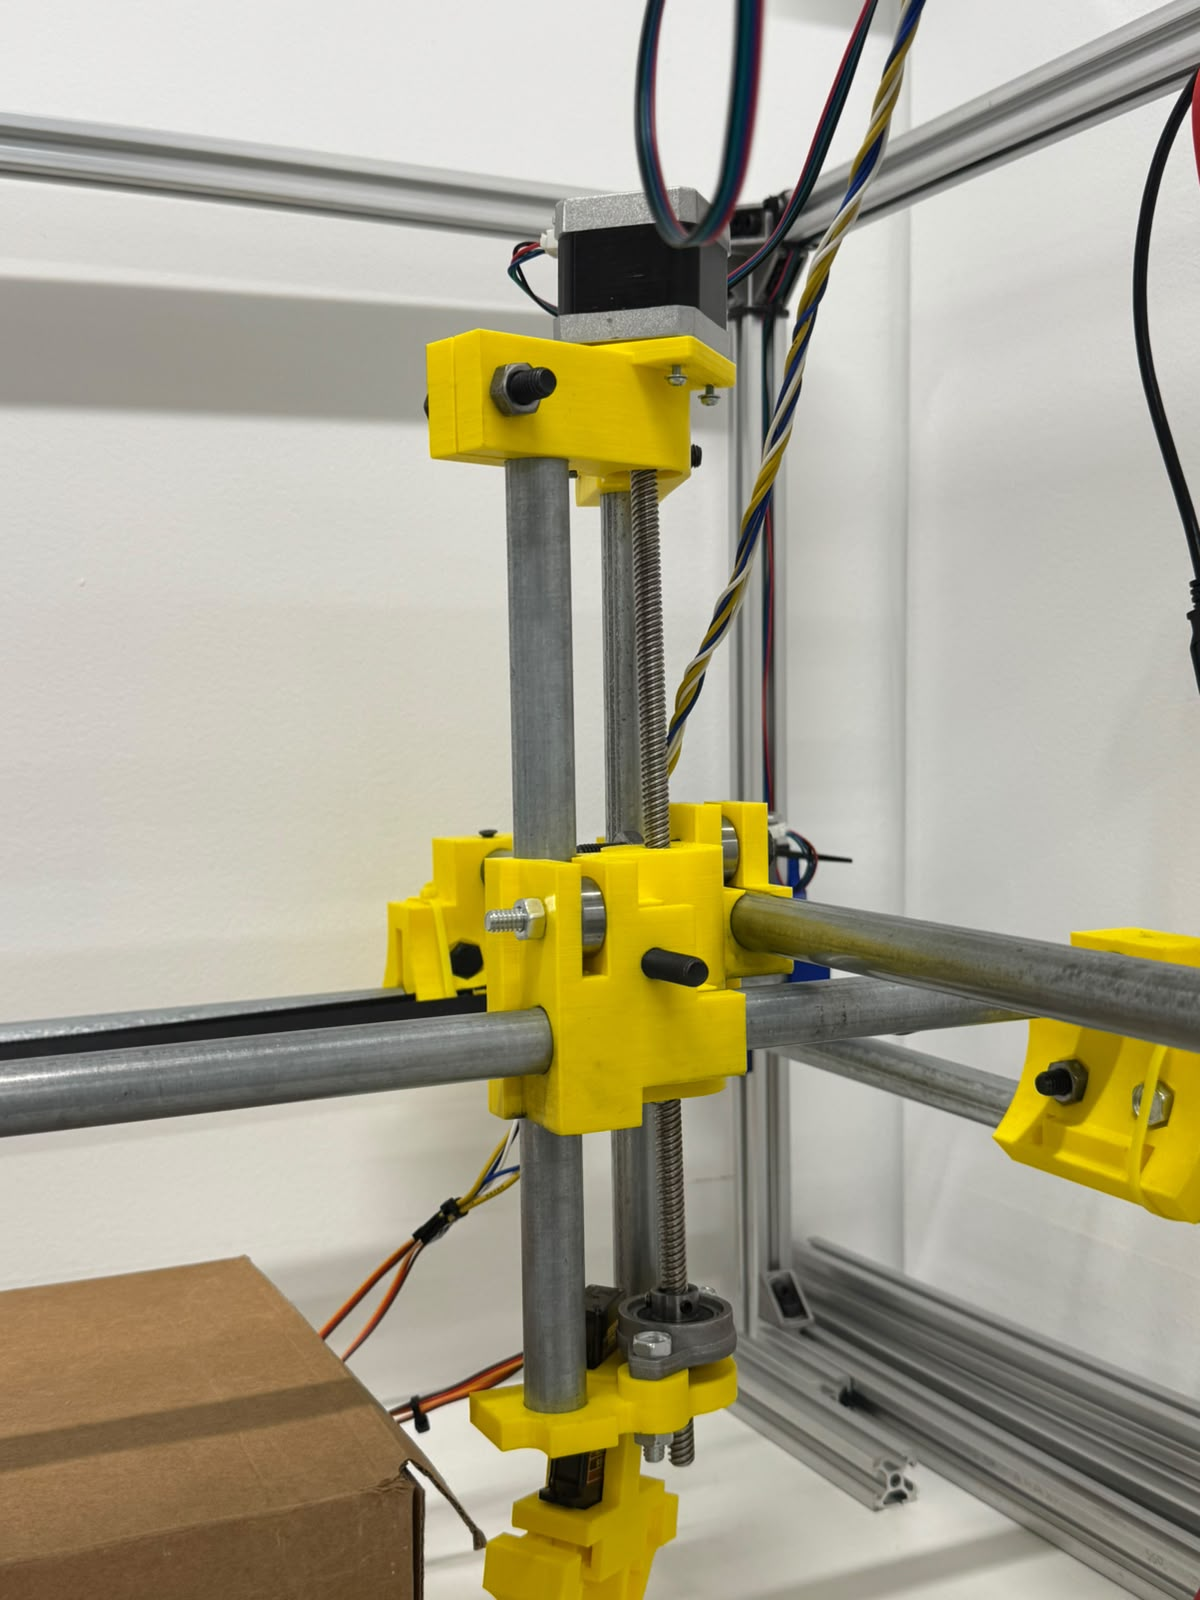
\includegraphics[width=0.55\textwidth,height=5.5cm,keepaspectratio]
    {Imagenes de Documentacion/F1_4.jpeg}
    \caption{Configuración inicial del mecanismo del eje Z.}
    \label{fig:fase1_eje_z}
    \par\small Fuente: elaboración propia.
\end{figure}

\begin{table}[H]
    \centering
    \caption{Observaciones de la evaluación mecánica inicial.}
    \label{tab:fase1_deficiencias}
    \begin{tabular}{p{0.08\textwidth}p{0.37\textwidth}p{0.43\textwidth}}
        \hline
        Eje & Configuración observada & Hallazgos de la inspección \\
        \hline
        X y Y &
        Carros impresos con rodamientos radiales sobre tubos metálicos. &
        Contacto plástico--tubo, resistencia al desplazamiento, desalineación y avance desigual de los extremos del pórtico. \\

        Z &
        Conjunto vertical con elementos de guiado y soportes impresos. &
        Desalineación del conjunto móvil y movimiento vertical irregular. \\
        \hline
    \end{tabular}
    \par\small\raggedright Fuente: elaboración propia a partir de la inspección visual y manual.
\end{table}


% ============================================================
% FASE 2
% ============================================================

\section{Fase 2. Selección de componentes y rediseño mecánico}
\label{sec:resultados_fase2}

Se obtuvo un modelo CAD que conservó la arquitectura cartesiana y la disposición general de los ejes X, Y y Z. Se adaptaron los diseños de los soportes de las guías y de los motores de X y Y para incorporar ejes de acero de 12~mm de diámetro. La fabricación de las piezas correspondió a la fase siguiente.

El diseño incluyó cuatro carros para X y Y con rodamientos lineales con carcasa. Cada carro incorporó un paso perpendicular para el eje correspondiente, un espacio para el recorrido de la faja dentada y dos puntos adicionales de fijación (Figura~\ref{fig:fase2_carro_xy}).

\begin{figure}[H]
    \centering
    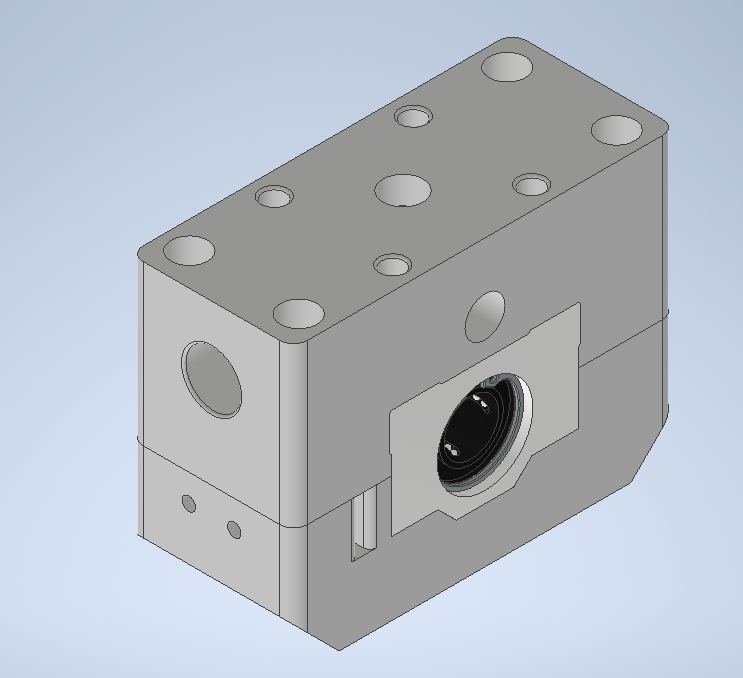
\includegraphics[width=0.65\textwidth,height=5.5cm,keepaspectratio]
    {Imagenes de Documentacion/F2_1.png}
    \caption{Modelo CAD del carro de traslación de los ejes X y Y.}
    \label{fig:fase2_carro_xy}
    \par\small Fuente: elaboración propia.
\end{figure}

El conjunto central incorporó rodamientos lineales cilíndricos para el desplazamiento en el plano XY. La intersección de ambos ejes quedó ubicada en el centro del conjunto y constituyó la referencia de montaje del mecanismo vertical (Figura~\ref{fig:fase2_centro_xy}).

\begin{figure}[H]
    \centering
    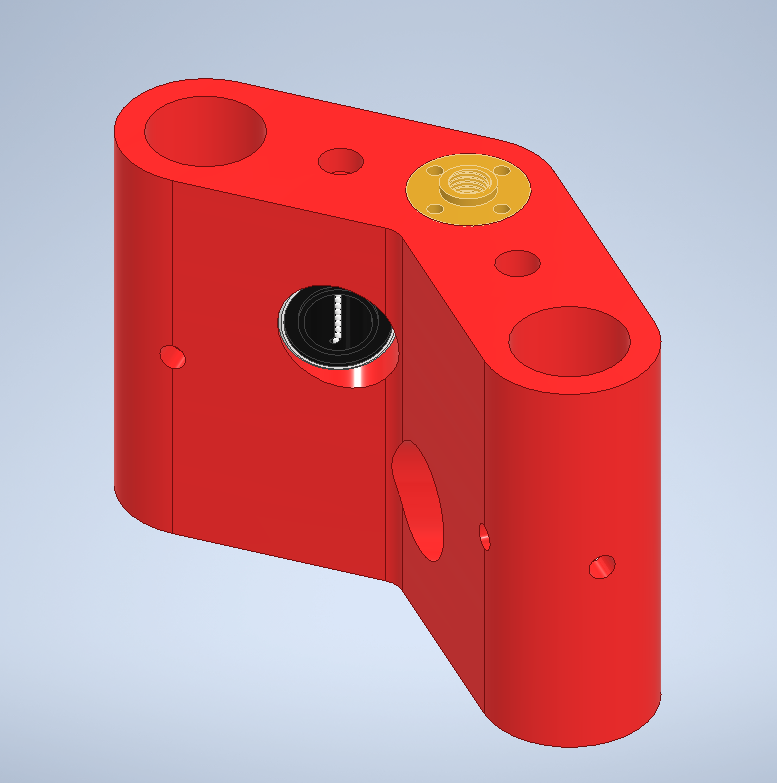
\includegraphics[width=0.65\textwidth,height=5.5cm,keepaspectratio]
    {Imagenes de Documentacion/F2_2.png}
    \caption{Modelo CAD del conjunto central del mecanismo cartesiano.}
    \label{fig:fase2_centro_xy}
    \par\small Fuente: elaboración propia.
\end{figure}

En el ensamblaje digital, Z incorporó dos guías y un tornillo de avance. Los soportes superior e inferior mantuvieron la separación entre centros definida en el conjunto central (Figura~\ref{fig:fase2_eje_z}). La integración de los componentes se documentó en el ensamblaje general de Autodesk Inventor (Figura~\ref{fig:fase2_ensamble_final}).

\begin{figure}[H]
    \centering
    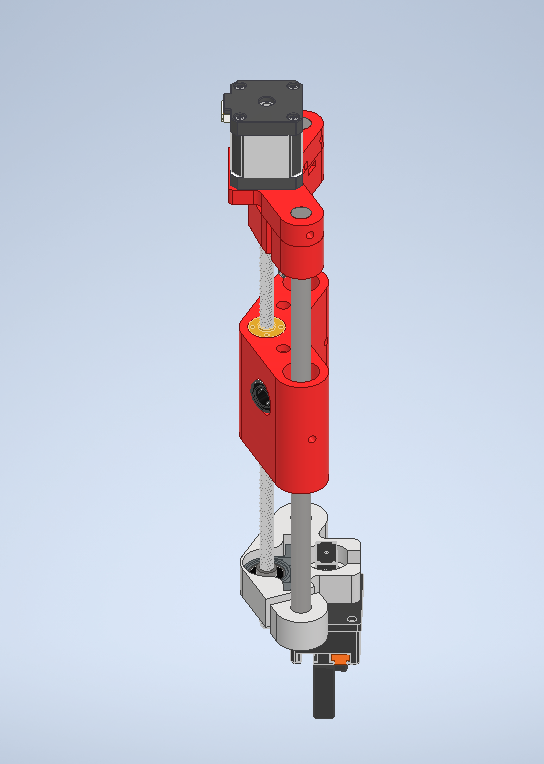
\includegraphics[width=0.60\textwidth,height=6cm,keepaspectratio]
    {Imagenes de Documentacion/F2_3.png}
    \caption{Modelo CAD del mecanismo vertical integrado al conjunto central.}
    \label{fig:fase2_eje_z}
    \par\small Fuente: elaboración propia.
\end{figure}

\begin{figure}[H]
    \centering
    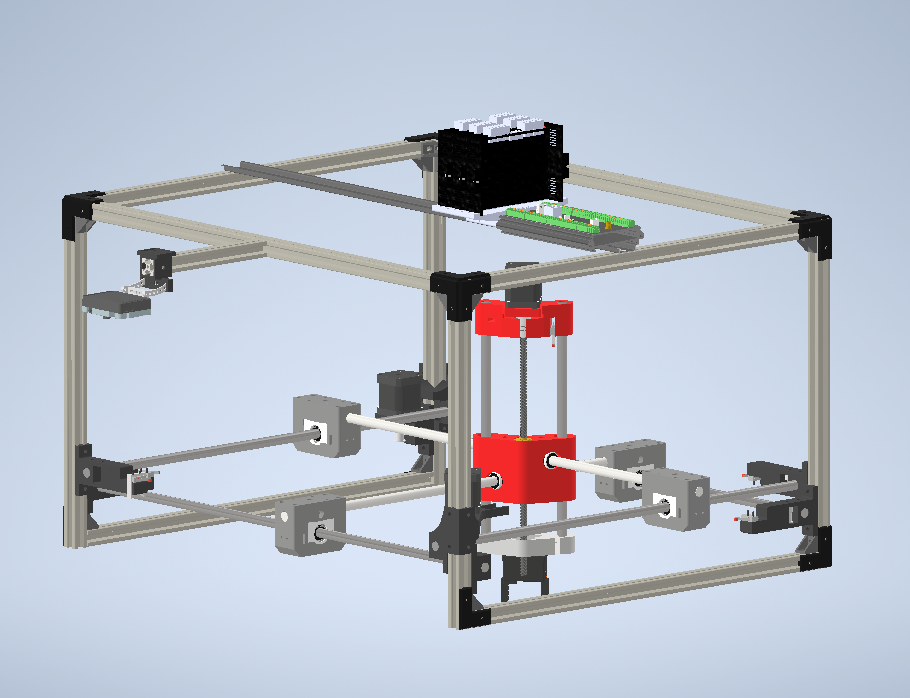
\includegraphics[width=0.75\textwidth,height=6cm,keepaspectratio]
    {Imagenes de Documentacion/F2_4.png}
    \caption{Ensamblaje CAD del brazo robótico cartesiano en Autodesk Inventor.}
    \label{fig:fase2_ensamble_final}
    \par\small Fuente: elaboración propia.
\end{figure}

% PENDIENTE:
% Confirmar si las imágenes CAD corresponden a la versión previa a fabricar
% o a una actualización posterior.


% ============================================================
% FASE 3
% ============================================================

\section{Fase 3. Implementación mecánica}
\label{sec:resultados_fase3}

\subsection{Componentes fabricados y configuración ensamblada}

Se incorporaron 48 piezas impresas en PLA, incluidas las escuadras de acabado estético. El consumo aproximado de material fue de 1.5~kg, incluidas las pruebas y las iteraciones de fabricación. Todas las piezas impresas se fabricaron nuevamente, incluso aquellas cuyos diseños se retomaron del mecanismo original.

Las piezas obtenidas incluyeron soportes de ejes guía, soportes de montaje de motores, carros de desplazamiento, piezas del conjunto central y soportes de Z. Parte de estos componentes se documentó en la Figura~\ref{fig:fase3_fabricacion}.

\begin{figure}[H]
    \centering
    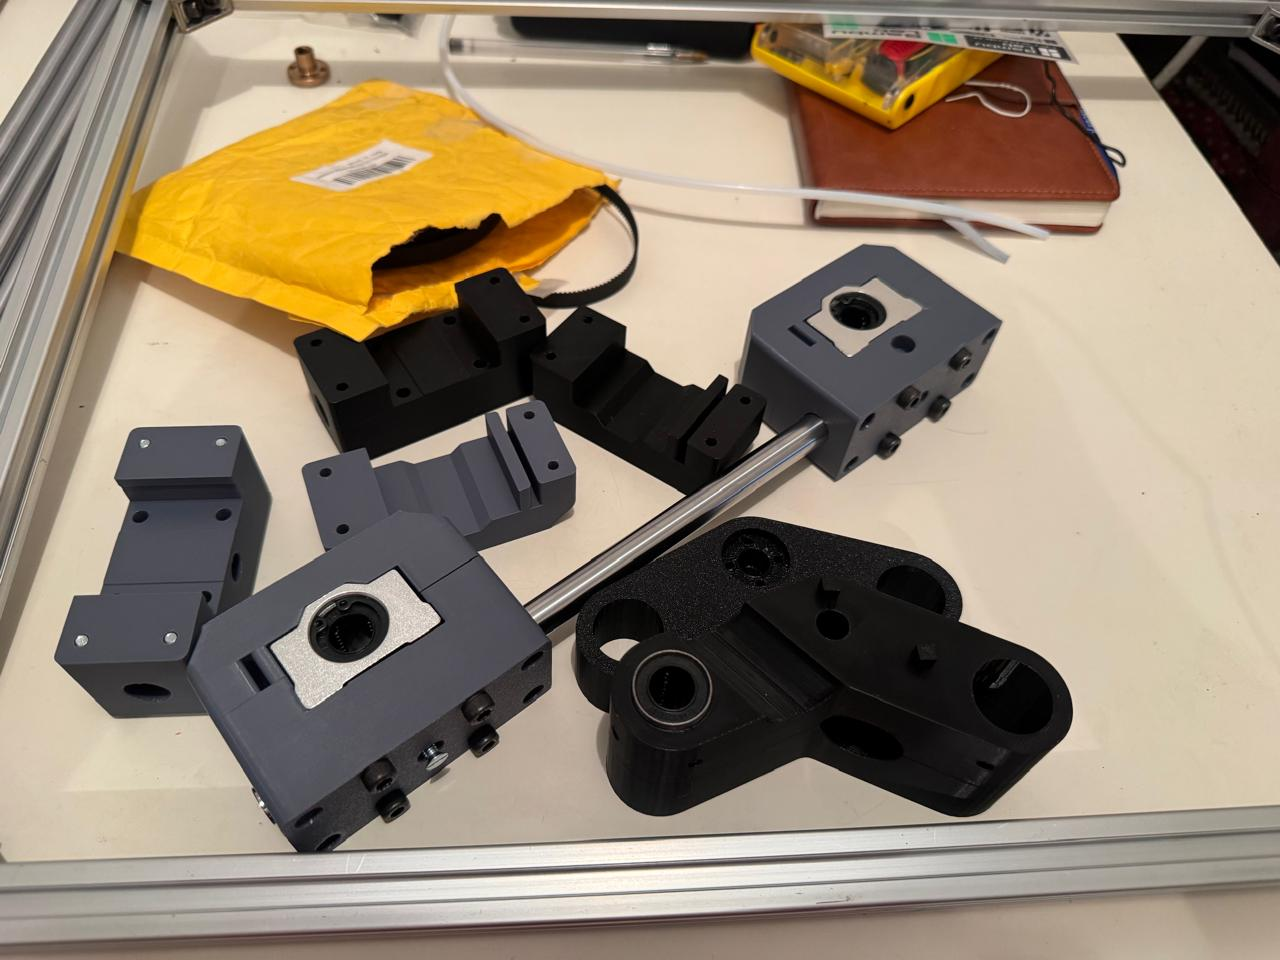
\includegraphics[width=0.72\textwidth,height=6cm,keepaspectratio]
    {figuras/fase3_componentes.jpeg}
    \caption{Componentes impresos y rodamientos preparados para el ensamblaje.}
    \label{fig:fase3_fabricacion}
    \par\small Fuente: elaboración propia.
\end{figure}

El conjunto ensamblado incorporó perfiles de aluminio 2020 de ranura en T, guías de acero de 12~mm, rodamientos lineales, fajas dentadas para X y Y y un tornillo de avance para Z. Las dimensiones y cantidades reportadas se organizaron en el Cuadro~\ref{tab:fase3_caracteristicas}.

\begin{table}[H]
    \centering
    \caption{Características del conjunto mecánico implementado.}
    \label{tab:fase3_caracteristicas}
    \begin{tabular}{p{0.53\textwidth}p{0.36\textwidth}}
        \hline
        Característica & Valor o configuración \\
        \hline
        Dimensiones generales de la estructura & $700 \times 580 \times 420$~mm \\
        Recorrido reportado del eje X\textsuperscript{a} & 446~mm \\
        Recorrido reportado del eje Y\textsuperscript{a} & 336~mm \\
        Recorrido del eje Z\textsuperscript{b} & 14\,687 pasos \\
        Diámetro de los ejes guía & 12~mm \\
        Ejes de 700~mm & 3 unidades \\
        Ejes de 580~mm & 3 unidades \\
        Perfiles estructurales & Aluminio 2020 de ranura en T \\
        Piezas impresas incorporadas & 48 unidades \\
        Material de las piezas impresas & PLA \\
        Consumo aproximado de PLA, incluidas las pruebas & 1.5~kg \\
        Transmisión en X y Y & Fajas dentadas \\
        Transmisión en Z & Tornillo de avance \\
        \hline
    \end{tabular}

    \par\small\raggedright Fuente: elaboración propia a partir de los datos de fabricación y ensamblaje del proyecto.
    \par\small La altura se refirió a la superficie de la mesa. El consumo de PLA incluyó las pruebas y no correspondió a la masa del brazo ensamblado.
    \par\small\textsuperscript{a} Se conservaron los valores reportados; su procedencia, del modelo CAD o de medición física, quedó pendiente de confirmación.
    \par\small\textsuperscript{b} Promedio de nueve referenciaciones registradas; no se implementó la conversión de Z a milímetros.
\end{table}


\subsection{Configuraciones del conjunto central y del soporte de la garra}

El conjunto central pasó por tres iteraciones. En las dos primeras se presentaron dificultades de retención de los rodamientos; en la configuración final estos permanecieron en sus alojamientos durante las comprobaciones de movimiento. Las configuraciones y sus observaciones se resumieron en el Cuadro~\ref{tab:fase3_iteraciones}.

\begin{table}[H]
    \centering
    \caption{Iteraciones del conjunto central y observaciones de montaje.}
    \label{tab:fase3_iteraciones}
    \begin{tabular}{p{0.10\textwidth}p{0.38\textwidth}p{0.40\textwidth}}
        \hline
        Iteración & Configuración & Observación \\
        \hline
        Primera &
        Cuerpo inicial al que se añadieron tornillos de presión. &
        Se observó la salida de los rodamientos de sus alojamientos antes de incorporar los tornillos. \\

        Segunda &
        Conjunto dividido en tres piezas con tornillos de presión. &
        Persistieron las dificultades de sujeción de los rodamientos. \\

        Tercera &
        Conjunto con tornillos de unión entre las piezas. &
        Los rodamientos permanecieron en sus alojamientos durante las comprobaciones realizadas. \\
        \hline
    \end{tabular}

    \par\small\raggedright Fuente: elaboración propia a partir de la descripción del proceso de fabricación y ensamblaje.
\end{table}

El conjunto central ensamblado y una vista del montaje parcial se documentaron en la Figura~\ref{fig:fase3_montaje}. El soporte inferior de Z incorporó una unión desmontable para la garra, en sustitución de la unión fija inicial. El efector final quedó ubicado en la intersección de los ejes del conjunto central.

\begin{figure}[H]
    \centering
    \begin{minipage}[b]{0.38\textwidth}
        \centering
        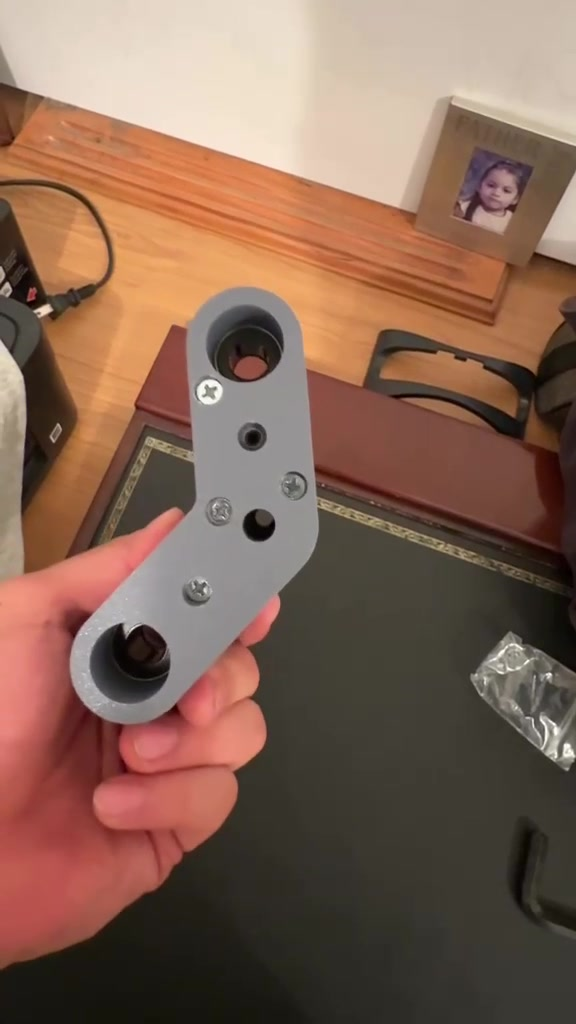
\includegraphics[width=\linewidth,height=6.5cm,keepaspectratio]
        {figuras/fase3_central_inferior.jpg}
        \par\small (a) Conjunto central ensamblado.
    \end{minipage}
    \hfill
    \begin{minipage}[b]{0.58\textwidth}
        \centering
        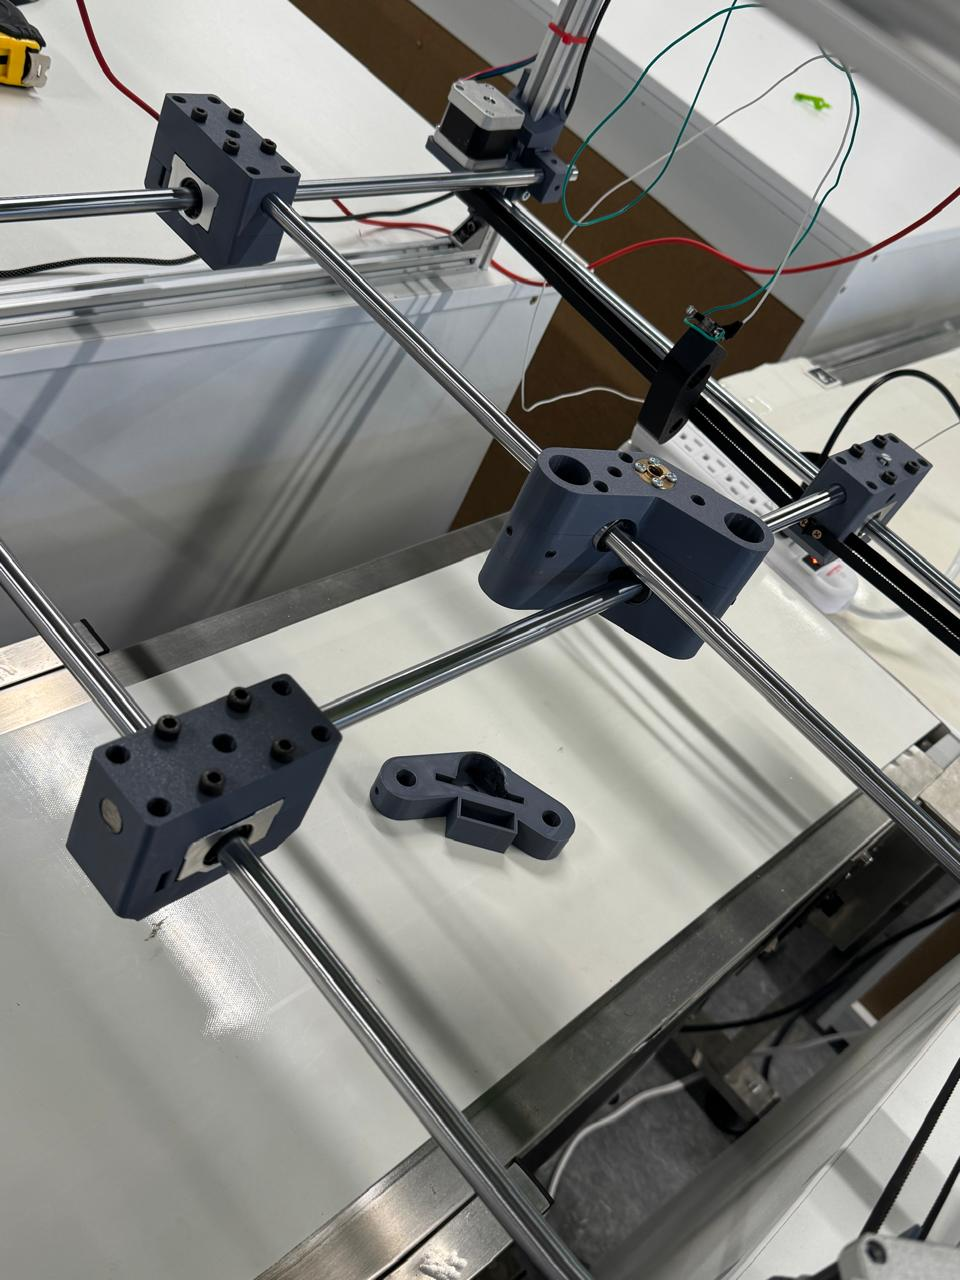
\includegraphics[width=\linewidth,height=6.5cm,keepaspectratio]
        {figuras/fase3_ensamblaje_parcial.jpeg}
        \par\small (b) Montaje parcial de guías y carros.
    \end{minipage}

    \caption{Conjunto central y montaje parcial del mecanismo cartesiano.}
    \label{fig:fase3_montaje}
    \par\small Fuente: elaboración propia; fotografía y fotograma del registro audiovisual del proyecto.
\end{figure}


\subsection{Comprobación mecánica preliminar}

Se comprobó el desplazamiento de los tres ejes mediante manipulación directa, antes del accionamiento electrónico. Los carros permanecieron sobre sus guías y no se reprodujeron los atascos identificados en el mecanismo original durante las comprobaciones realizadas.

La resistencia al movimiento se percibió menor que en el sistema original. El avance desigual de los extremos del pórtico resultó poco perceptible durante la inspección visual. Se observaron vibraciones leves y no se identificó deflexión de las guías a simple vista.

Estas observaciones fueron cualitativas y no correspondieron a mediciones de precisión o repetibilidad.


% ============================================================
% FASE 4
% ============================================================

\section{Fase 4. Accionamiento electrónico, operación manual y referenciación}
\label{sec:resultados_fase4}

\subsection{Arquitectura electrónica y accionamiento implementado}

La integración electrónica dio como resultado una arquitectura de control distribuida entre la ESP32 y la Portenta H7 con Machine Control. La Portenta concentró la generación de las señales STEP y DIR de los tres motores paso a paso, la lectura de los seis finales de carrera, el conteo de pasos, la referenciación y la coordinación de los estados generales del brazo. La ESP32 concentró la lectura del mando inalámbrico, el accionamiento de los dos servomotores, la interfaz mediante la pantalla OLED y, en la fase posterior, la comunicación con el sistema de visión.

Durante el desarrollo inicial, la electrónica se comprobó en protoboards. Esta configuración correspondió a la etapa de prototipado y permitió integrar de manera conjunta el accionamiento de los ejes, los finales de carrera, los microcontroladores, los servomotores y los periféricos antes de realizar el montaje permanente en placas perforadas.

La Figura~\ref{fig:BrazoProto} muestra el brazo cartesiano durante esta etapa de integración. En las tres vistas se observa la estructura instalada sobre la banda transportadora y la distribución temporal de los módulos electrónicos sobre la parte superior del sistema.

\begin{figure}[H]
    \centering

    \begin{minipage}[b]{0.48\textwidth}
        \centering
        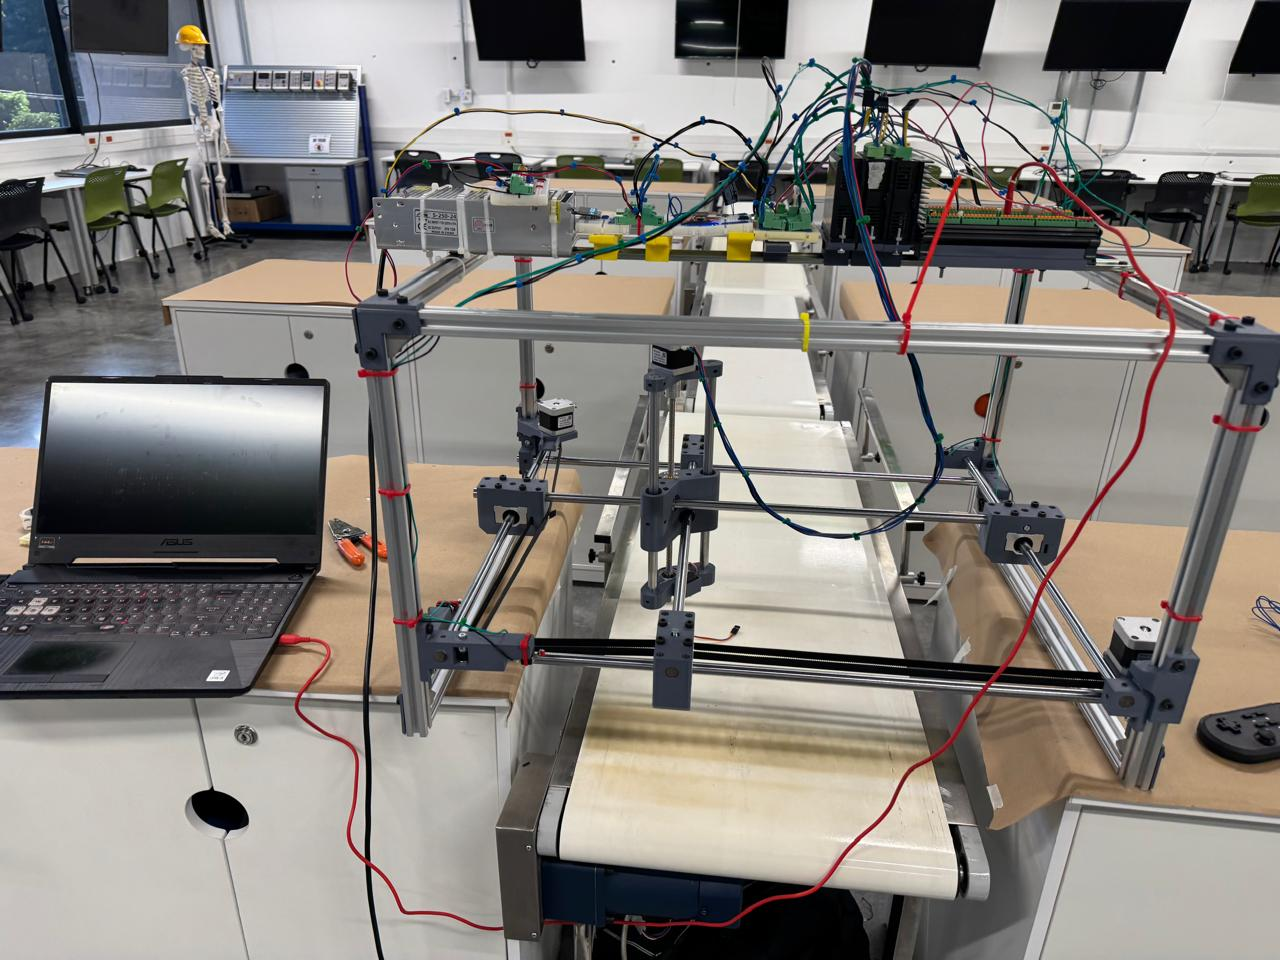
\includegraphics[
            width=\linewidth,
            height=7cm,
            keepaspectratio
        ]{Imagenes de Documentacion/BrazoProto1.jpeg}
        \par\small (a)
    \end{minipage}
    \hfill
    \begin{minipage}[b]{0.48\textwidth}
        \centering
        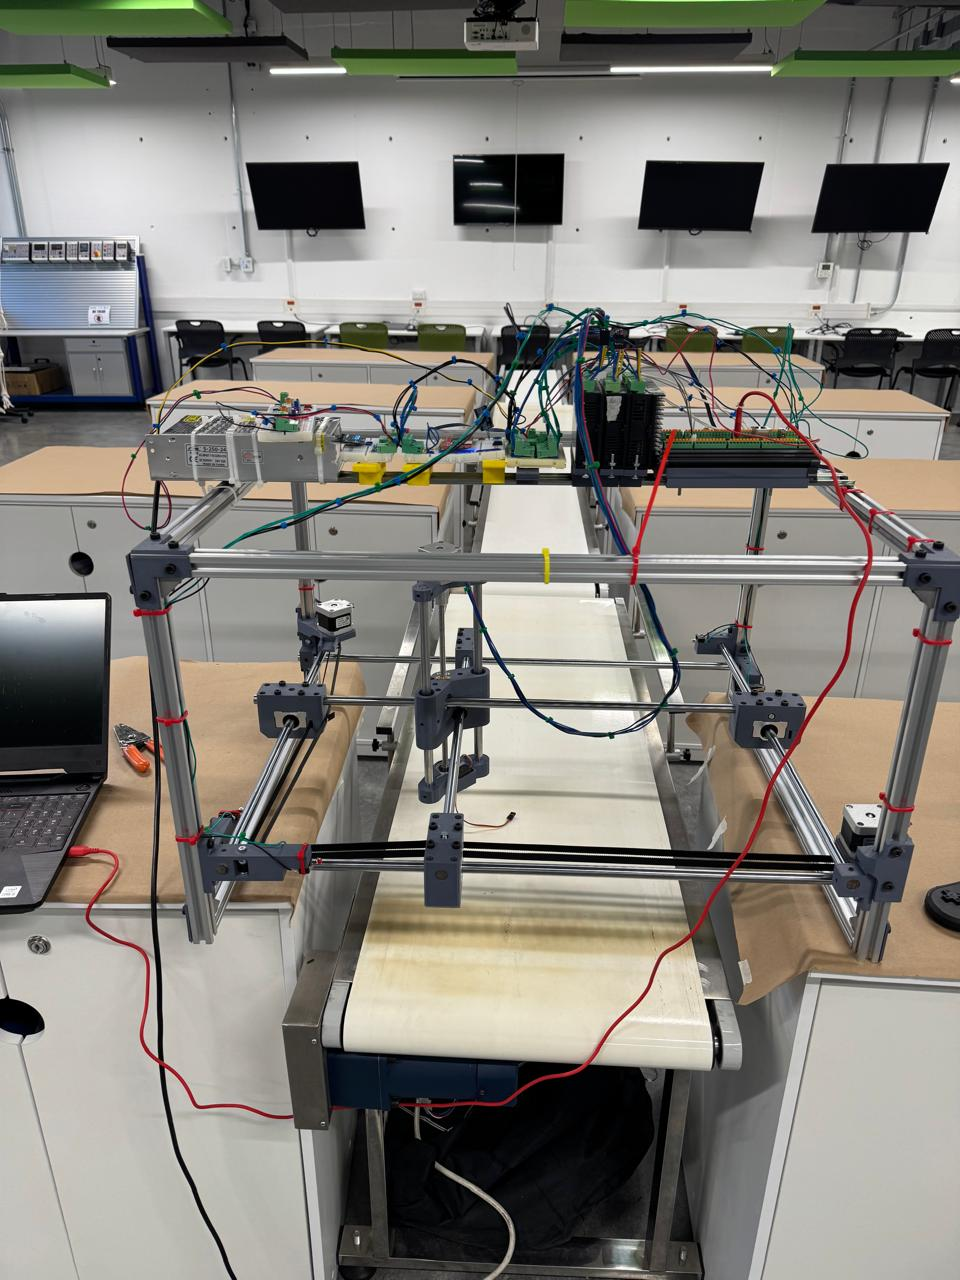
\includegraphics[
            width=\linewidth,
            height=7cm,
            keepaspectratio
        ]{Imagenes de Documentacion/BrazoProto2.jpeg}
        \par\small (b)
    \end{minipage}

    \par\medskip

    \begin{minipage}[c]{0.62\textwidth}
        \centering
        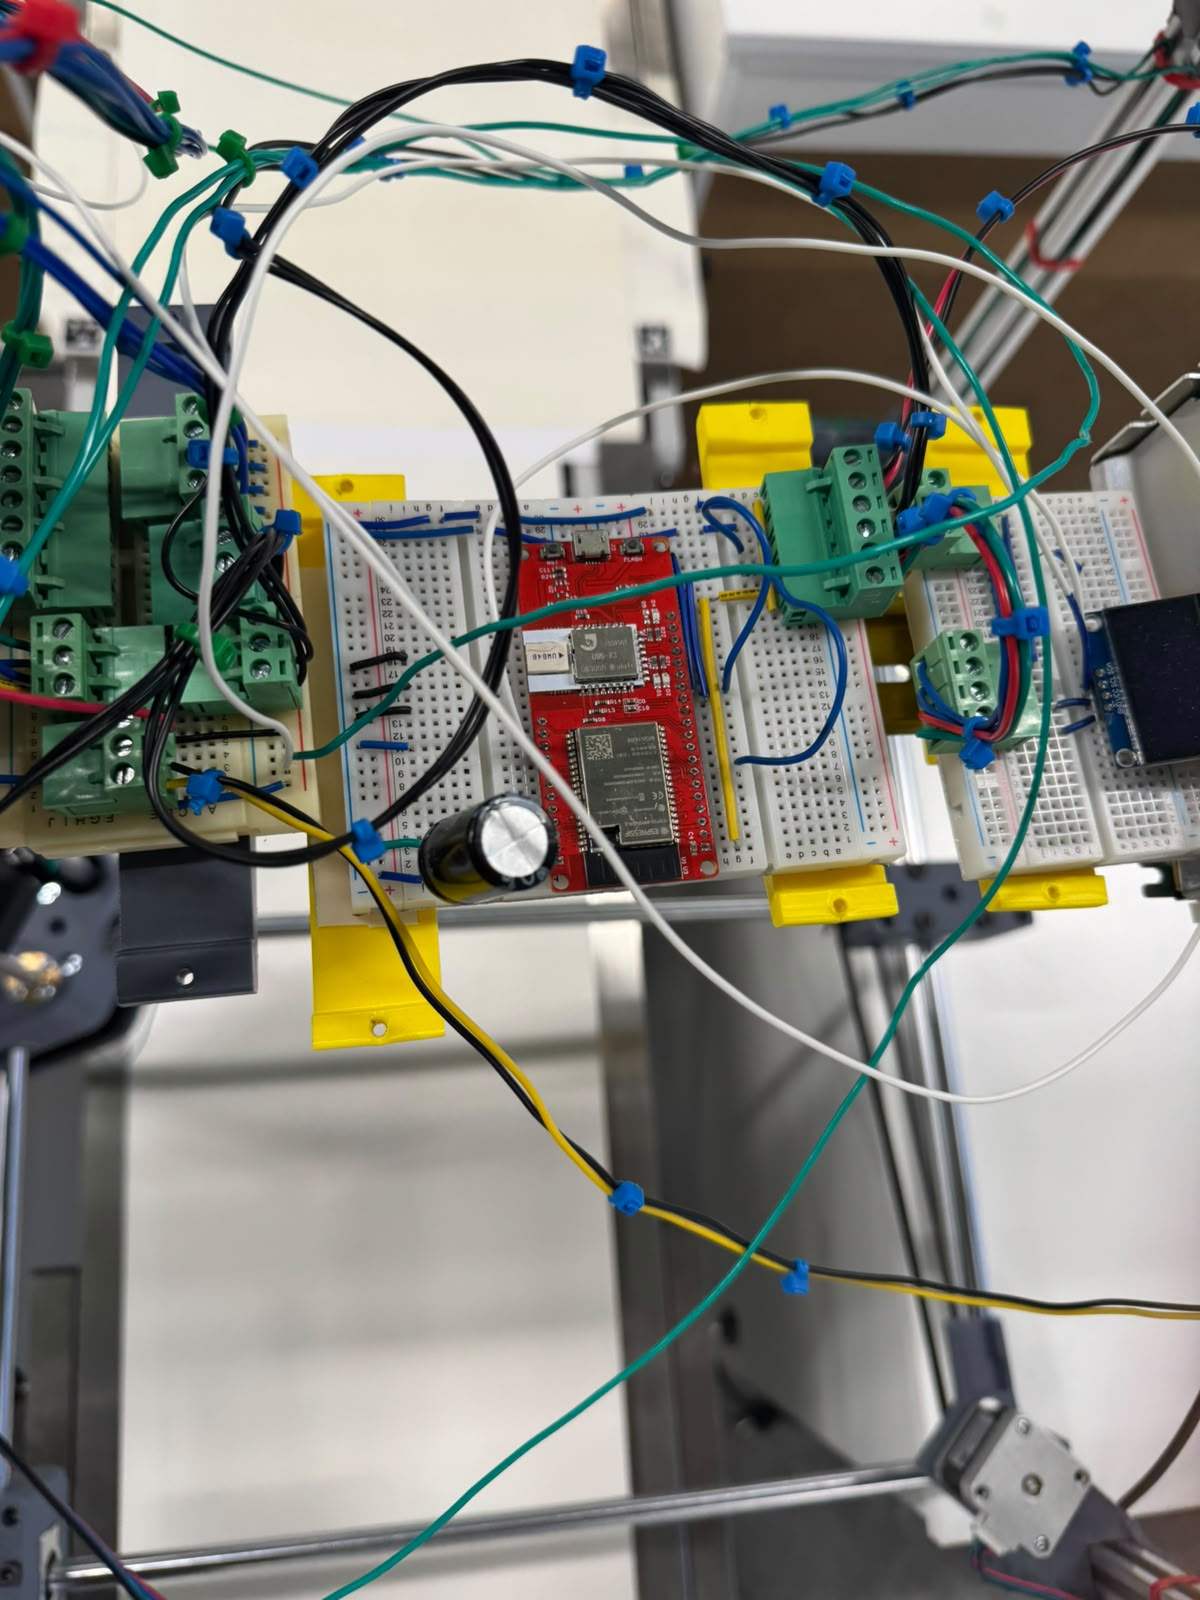
\includegraphics[
            width=\linewidth,
            height=7cm,
            keepaspectratio
        ]{Imagenes de Documentacion/BrazoProto3.jpeg}
        \par\small (c)
    \end{minipage}

    \caption{Montaje electrónico temporal utilizado durante las pruebas de integración en protoboards. (a) Vista frontal del brazo cartesiano. (b) Vista general del sistema durante las pruebas de integración. (c) Distribución de los módulos durante la etapa de prototipado.}
    \label{fig:BrazoProto}

    \par\small Fuente: elaboración propia.
\end{figure}

El accionamiento permitió desplazar los ejes X, Y y Z en ambos sentidos dentro de los límites habilitados por el sistema. La activación de un final de carrera bloqueó el desplazamiento hacia el extremo correspondiente y mantuvo disponible el movimiento en el sentido contrario para liberar el sensor. La lectura conjunta de los finales también permitió identificar como incoherente la activación simultánea de los dos límites de un mismo eje.

La distribución funcional obtenida se resumió en el Cuadro~\ref{tab:fase4_resultado_arquitectura}.

\begin{table}[H]
    \centering
    \caption{Distribución funcional obtenida en la arquitectura electrónica.}
    \label{tab:fase4_resultado_arquitectura}
    \begin{tabular}{p{0.27\textwidth}p{0.61\textwidth}}
        \hline
        Subsistema & Funciones integradas \\
        \hline
        Portenta H7 con Machine Control &
        Accionamiento X/Y/Z, lectura de finales de carrera, conteo de pasos, referenciación, posicionamiento y coordinación de estados. \\

        ESP32 &
        Mando inalámbrico, pantalla OLED, control de los dos servomotores, enlace con la cámara y procesamiento visual. \\

        Efector final &
        Rotación y apertura/cierre mediante dos servomotores controlados por la ESP32. \\

        Interfaz local &
        Presentación de estados, menús, calibración y variables de operación mediante la pantalla OLED. \\
        \hline
    \end{tabular}

    \par\small\raggedright Fuente: elaboración propia a partir de la implementación integrada del sistema.
\end{table}


\subsection{Comunicación entre la Portenta H7 y la ESP32}

En la implementación inicial se obtuvo un intercambio bidireccional de información entre la Portenta H7 y la ESP32 mediante I2C. La Portenta operó como maestra y la ESP32 como esclava en la dirección \texttt{0x40}, con una frecuencia de bus de 100~kHz. La pantalla OLED permaneció en un bus I2C independiente administrado por la ESP32.

El protocolo de aplicación empleó paquetes de 32 bytes en ambos sentidos. El intercambio permitió enviar desde la ESP32 las órdenes del mando, estados del efector final y variables asociadas con la cámara, mientras que la Portenta devolvió el estado general, los límites, los movimientos y, posteriormente, la información del encoder.

El formato incorporó comprobaciones de identificación, versión, longitud, CRC, secuencia y vigencia antes de aceptar los datos.

Durante esta etapa, el enlace permitió que las órdenes originadas en el mando fueran ejecutadas por la Portenta y que la ESP32 recibiera el estado resultante para actualizar la interfaz. Su comportamiento durante el montaje permanente y la posterior sustitución por UART sobre RS485 se presentan en las subsecciones siguientes.


\subsection{Operación manual e interfaz de usuario}

El modo manual permitió comandar los desplazamientos de X, Y y Z mediante el mando inalámbrico. Los movimientos se mantuvieron mientras la entrada correspondiente permaneció fuera de la zona neutra y se detuvieron al regresar el joystick a la posición central, al salir del modo o cuando un final de carrera bloqueó el sentido solicitado.

El mismo mando permitió modificar la orientación del efector final y alternar la apertura y el cierre de la pinza. El servo de rotación se controló mediante el eje horizontal del joystick derecho y la pinza se alternó mediante el botón correspondiente del mando.

La pérdida de conexión del control produjo la neutralización de las órdenes de movimiento.

La pantalla OLED presentó los estados principales del sistema, los modos disponibles, la fase de calibración, las direcciones de movimiento y la información utilizada por el operador durante la operación.

Estas funciones permitieron disponer de un modo de operación manual independiente del posicionamiento cartesiano por coordenadas.


\subsection{Referenciación y posicionamiento cartesiano}

La rutina de referenciación integró los tres ejes y estableció un origen común en el centro del recorrido contado de X, Y y Z. Después de recorrer los extremos y finalizar el centrado, los contadores internos de los tres ejes se restablecieron a cero.

Para X y Y se utilizaron recorridos físicos configurados de 446~mm y 336~mm, respectivamente. A partir del número de pasos contado entre los extremos se calcularon los factores de conversión empleados por el posicionamiento cartesiano.

Después de la referenciación, el sistema permitió introducir destinos absolutos de X y Y y convertirlos a posiciones en pasos.

El movimiento cartesiano se mantuvo separado del movimiento manual: el primero utilizó destinos absolutos, mientras que el segundo utilizó órdenes direccionales continuas.

El eje Z quedó integrado en la calibración, el modo manual, el retorno a la posición de referencia y las secuencias automáticas de captura. Sin embargo, no se implementó una conversión de Z en milímetros equivalente a la utilizada para X y Y.

En las referenciaciones registradas, el recorrido medio entre finales de carrera fue de 19\,944,5 pasos en X, 11\,811,9 pasos en Y y 14\,687,2 pasos en Z. Con las longitudes configuradas, los factores medios fueron de 44,72~pasos/mm en X y 35,15~pasos/mm en Y, equivalentes a una resolución de 0,022~mm y 0,028~mm por paso, respectivamente. La dispersión de estas mediciones se presenta en la Sección~\ref{sec:resultados_repetibilidad}.


\subsection{Montaje permanente y comportamiento inicial del enlace I2C}

La implementación permanente quedó distribuida en cinco placas perforadas. Una placa se destinó a los convertidores reductores de tensión y a la alimentación de la cámara; una segunda, al control y alimentación de los servomotores; una tercera, a la distribución de 24~V y los conductores de retorno; una cuarta, a la ESP32 y sus interconexiones; y una quinta, a la conexión de la pantalla OLED para permitir su ubicación sobre la estructura.

La Figura~\ref{fig:fase4_montaje_permanente} muestra la distribución general de la electrónica después del traslado desde los protoboards hacia las placas perforadas.

\begin{figure}[H]
    \centering
    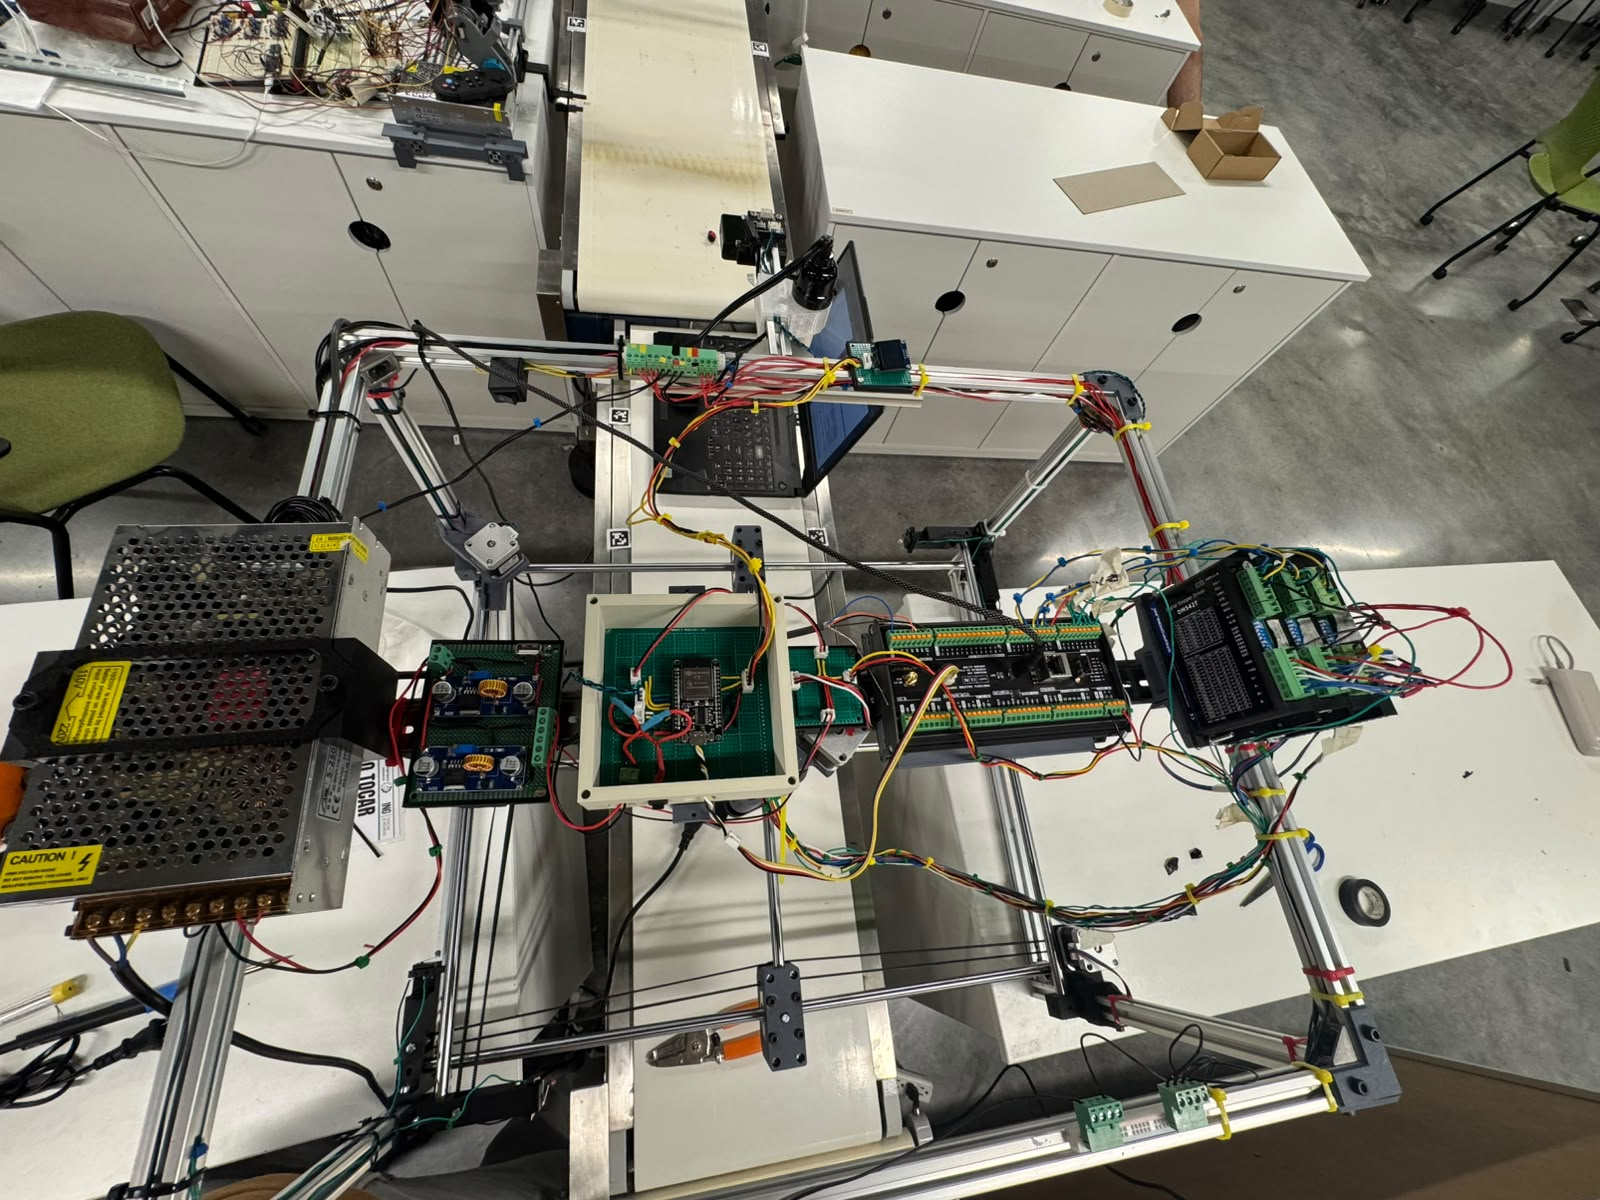
\includegraphics[
        width=0.90\textwidth,
        height=8.5cm,
        keepaspectratio
    ]{Imagenes de Documentacion/PCBgeneral.jpeg}
    \caption{Vista general de la implementación permanente del sistema electrónico sobre placas perforadas y su integración con la estructura del brazo cartesiano.}
    \label{fig:fase4_montaje_permanente}
    \par\small Fuente: elaboración propia.
\end{figure}

La distribución de los subsistemas permitió separar físicamente la regulación de alimentación de la placa que alojó la ESP32 y sus conexiones. La Figura~\ref{fig:fase4_placas_perforadas} muestra ambas secciones.

\begin{figure}[H]
    \centering

    \begin{minipage}[b]{0.48\textwidth}
        \centering
        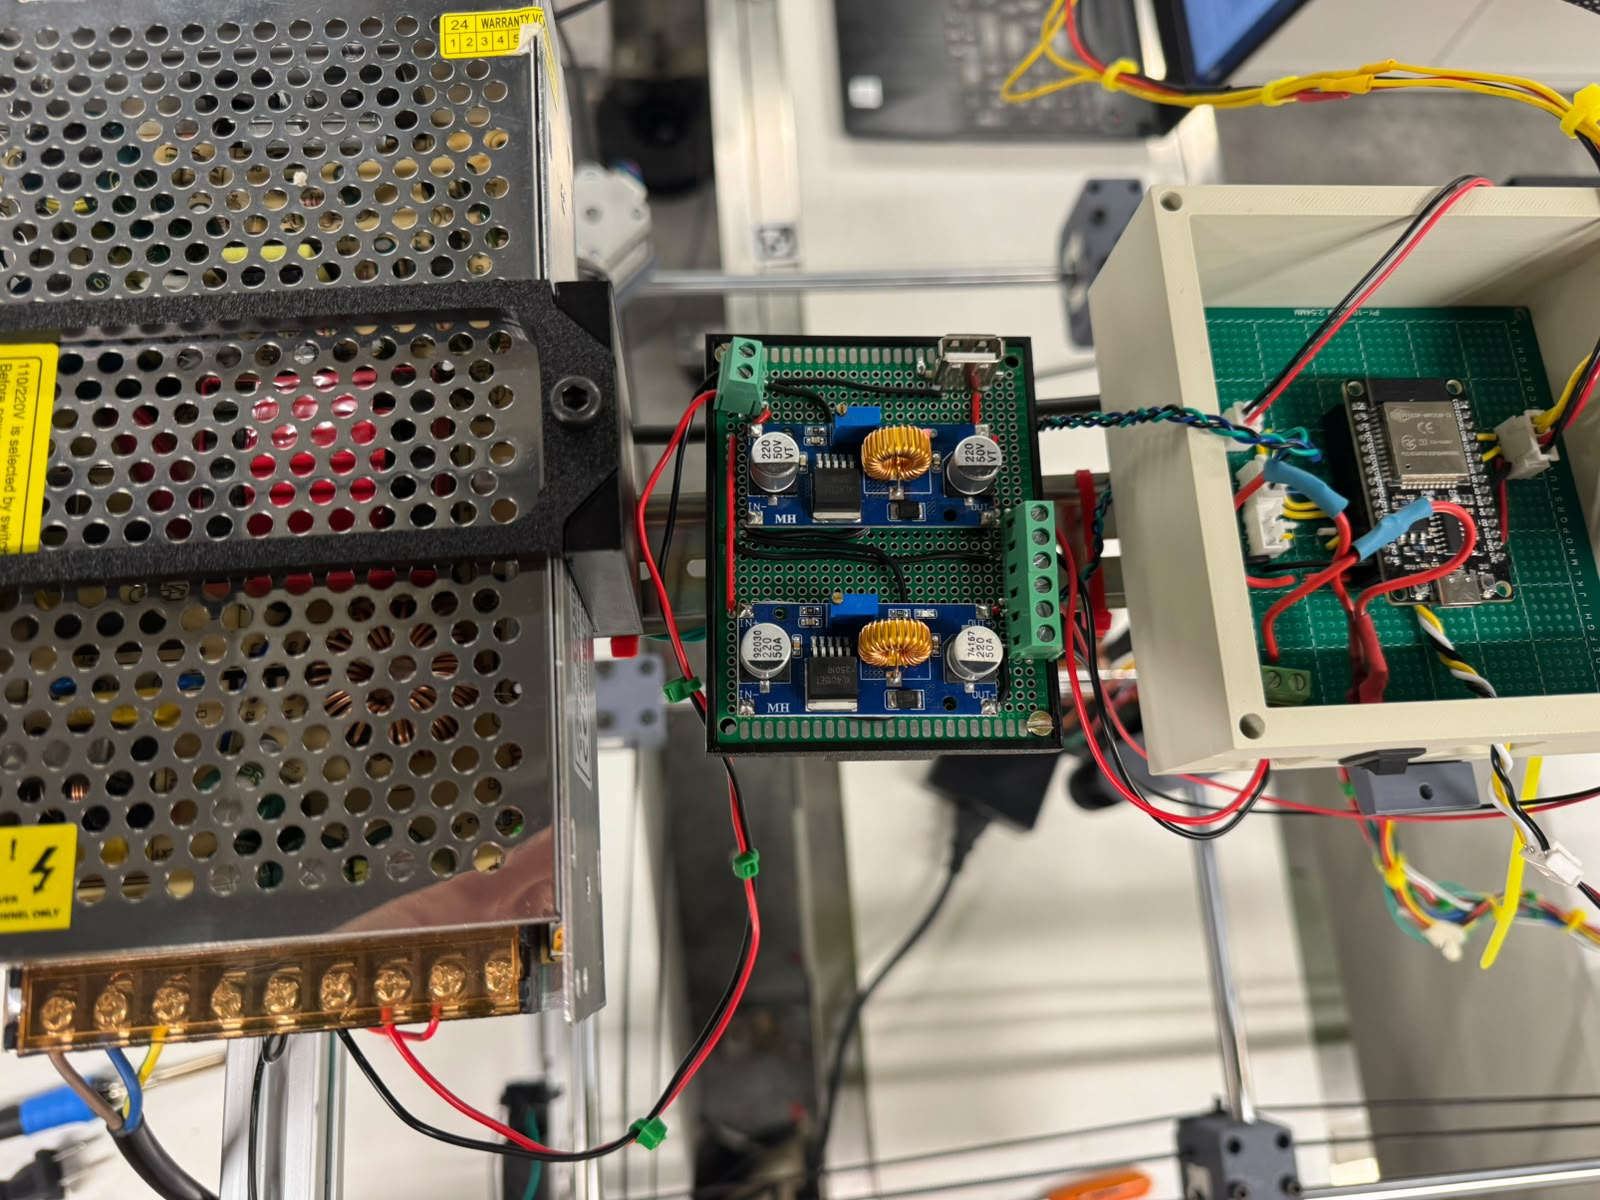
\includegraphics[
            width=\linewidth,
            height=6.5cm,
            keepaspectratio
        ]{Imagenes de Documentacion/ReguladoresFuente.jpeg}
        \par\small (a)
    \end{minipage}
    \hfill
    \begin{minipage}[b]{0.48\textwidth}
        \centering
        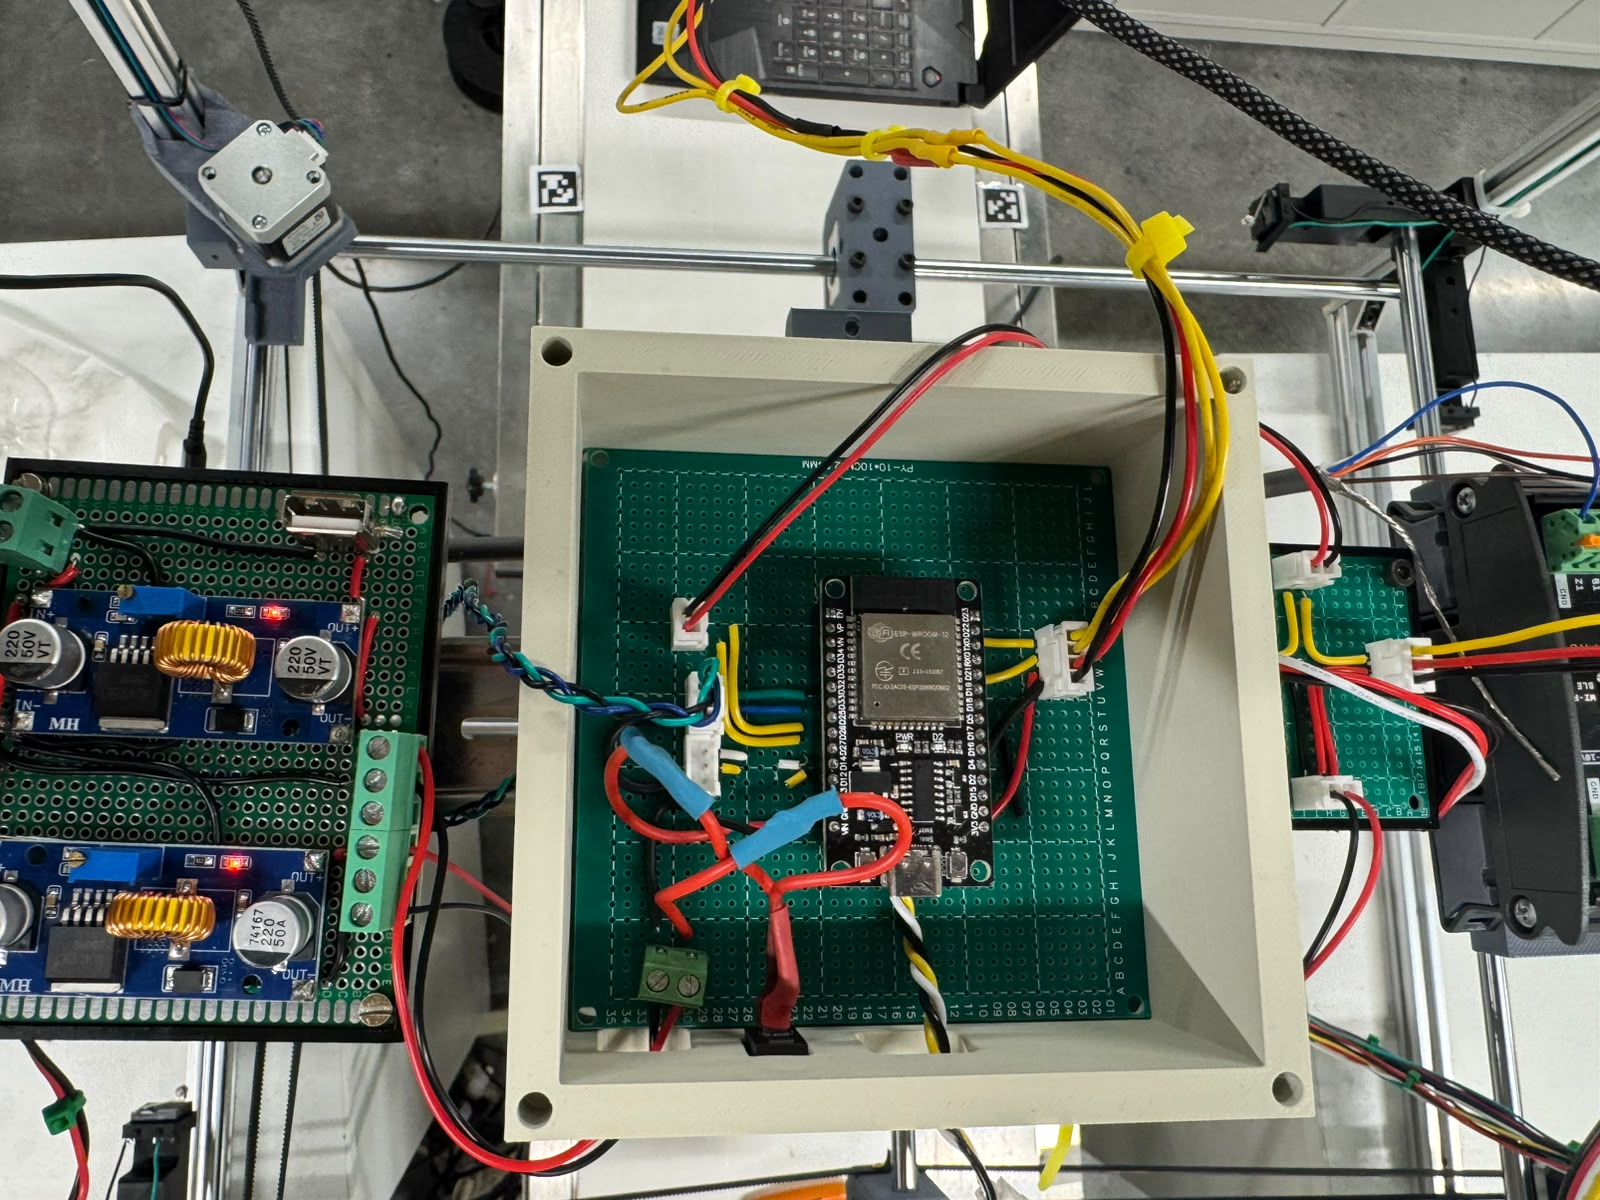
\includegraphics[
            width=\linewidth,
            height=6.5cm,
            keepaspectratio
        ]{Imagenes de Documentacion/Central.jpeg}
        \par\small (b)
    \end{minipage}

    \caption{Implementación de subsistemas sobre placas perforadas. (a) Placa destinada a los convertidores reductores de tensión y distribución de alimentación. (b) Placa que alojó la ESP32 y las interconexiones correspondientes a los periféricos y buses de comunicación.}
    \label{fig:fase4_placas_perforadas}
    \par\small Fuente: elaboración propia.
\end{figure}

La Portenta H7 con Machine Control y los controladores de los motores paso a paso permanecieron agrupados en la sección destinada al accionamiento de los tres ejes. La disposición obtenida se muestra en la Figura~\ref{fig:fase4_portenta_drivers}.

\begin{figure}[H]
    \centering
    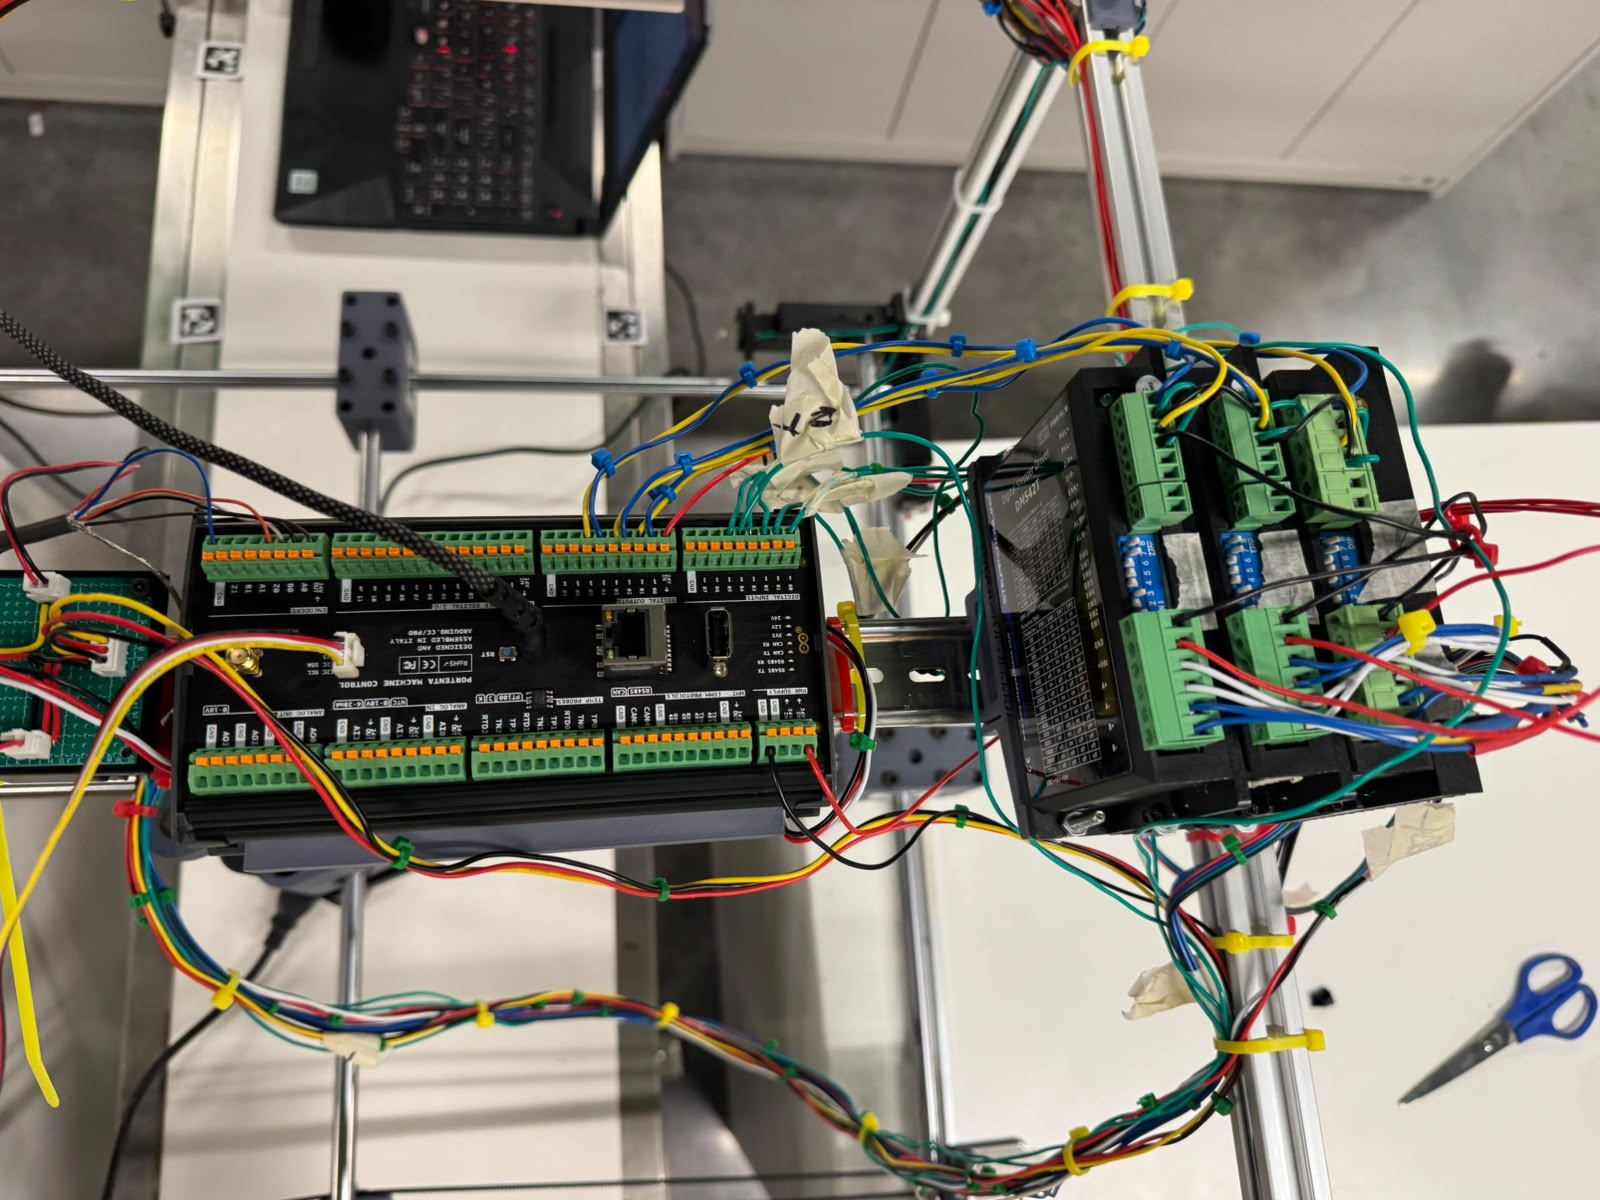
\includegraphics[
        width=0.80\textwidth,
        height=7.5cm,
        keepaspectratio
    ]{Imagenes de Documentacion/ConexionesDriversPortenta.jpeg}
    \caption{Integración de la Portenta H7 con Machine Control y los controladores de los motores paso a paso en el montaje permanente.}
    \label{fig:fase4_portenta_drivers}
    \par\small Fuente: elaboración propia.
\end{figure}

En la primera distribución física del montaje permanente, los conductores de alimentación, retorno y señal compartieron gran parte del recorrido central asociado con el riel DIN. Durante las comprobaciones con el sistema completo energizado se observaron paquetes inválidos o corruptos en el enlace I2C entre la Portenta H7 y la ESP32.

Después de reorganizar el cableado, los conductores de 24~V y los retornos a tierra se condujeron por trayectorias laterales opuestas y las líneas de señal se mantuvieron separadas de los grupos de potencia. En las comprobaciones inmediatamente posteriores a esta reorganización, el intercambio I2C presentó un comportamiento estable y dejaron de observarse las corrupciones de paquetes identificadas con la disposición anterior. Esta mejora correspondió a las verificaciones de esa etapa y no constituyó una validación definitiva de estabilidad durante la operación posterior.

El cambio observado se resumió en el Cuadro~\ref{tab:fase4_cableado_i2c}.

\begin{table}[H]
    \centering
    \caption{Comportamiento observado del enlace I2C durante la integración física.}
    \label{tab:fase4_cableado_i2c}
    \begin{tabular}{p{0.30\textwidth}p{0.29\textwidth}p{0.29\textwidth}}
        \hline
        Configuración & Distribución del cableado & Comportamiento observado \\
        \hline

        Montaje inicial en placas perforadas &
        Alimentación, retorno y señales concentrados en un recorrido central. &
        Se observaron paquetes inválidos o corruptos durante la operación del sistema completo. \\

        Montaje reorganizado &
        24~V y retornos por trayectorias laterales separadas; señales separadas de los grupos de potencia. &
        El enlace se mantuvo estable en las comprobaciones inmediatas a la reorganización del cableado. \\

        \hline
    \end{tabular}

    \par\small\raggedright Fuente: elaboración propia a partir de las comprobaciones realizadas durante la integración del prototipo.
\end{table}


\subsection{Persistencia de las fallas y migración a UART sobre RS485}

A pesar de la mejoría observada después de reorganizar los conductores, en comprobaciones posteriores del sistema integrado volvieron a presentarse dificultades de comunicación y recepción de paquetes inválidos o corruptos entre la Portenta H7 y la ESP32. Por consiguiente, la corrección inicial del cableado no resultó suficiente para considerar resuelta de forma definitiva la inestabilidad del enlace I2C.

Un registro de aproximadamente 30~s obtenido el 6 de octubre de 2026 durante una referenciación cuantificó el problema. En la captura completa fallaron el 10,7~\% de las lecturas de la Portenta (231 de 2158), el 15,7~\% de sus envíos (196 de 1250) y el 14,9~\% de las recepciones de la ESP32 (174 de 1165). Mientras se movía el eje Y, las tres tasas aumentaron a valores entre 22 y 30~\%, y la Portenta declaró la pérdida del enlace, detuvo el movimiento y reinició el periférico I2C. La ESP32 recibió longitudes de 1 a 31 bytes cuando se esperaban paquetes de 32 bytes.

Ante esta situación, se sustituyó la comunicación entre ambos microcontroladores por UART sobre RS485, según el procedimiento descrito en la metodología, manteniendo la distribución de tareas de la arquitectura electrónica. La conexión diferencial se realizó entre los terminales A/B del módulo MAX485 y los bornes TX P/TX N de Machine Control, utilizados para el intercambio bidireccional en modo \textit{half-duplex}. El Cuadro~\ref{tab:fase4_comparacion_enlace} resume las diferencias entre el enlace inicial y la configuración implementada posteriormente.

\begin{table}[H]
    \centering
    \caption{Configuración del enlace entre microcontroladores antes y después de la migración.}
    \label{tab:fase4_comparacion_enlace}
    \begin{tabular}{p{0.27\textwidth}p{0.30\textwidth}p{0.31\textwidth}}
        \hline
        Parámetro & Enlace inicial I2C & Enlace posterior UART sobre RS485 \\
        \hline
        Coordinación & Portenta maestra; ESP32 esclava en \texttt{0x40}. & Portenta inicia solicitudes; ESP32 responde. \\
        Señales en la ESP32 & SDA: GPIO27; SCL: GPIO14. & TX: GPIO27; RX: GPIO14; DE/\texttt{/RE}: GPIO18. \\
        Configuración & Bus I2C a 100~kHz. & UART a 115200 baudios, 8N1 y \textit{half-duplex}. \\
        Medio físico & Líneas SDA/SCL con resistencias de elevación. & Par diferencial A/B mediante MAX485 e interfaz RS485 de Machine Control. \\
        Información de aplicación & Paquetes de 32 bytes. & Paquetes de aplicación de 32 bytes, transportados en tramas de 44 bytes. \\
        \hline
    \end{tabular}
    \par\small\raggedright Fuente: elaboración propia a partir de las configuraciones documentadas en el firmware del sistema.
\end{table}

La versión final incorporó validaciones de integridad en dos capas: el CRC16 de la trama de transporte y el CRC-8 del paquete de aplicación de 32 bytes. La aplicación del nuevo enlace conservó el esquema de intercambio de estados completos: la Portenta transmitió sus estados y órdenes, mientras que la ESP32 devolvió el estado del mando, los servomotores y el sistema de visión. Para validar las respuestas se utilizaron la sesión y el identificador de solicitud, además de la comprobación de versión, longitud e integridad del paquete. Esta adaptación permitió mantener la comunicación funcional entre los controladores sin trasladar la pantalla OLED ni la cámara al bus diferencial; la primera conservó su conexión I2C con la ESP32 y la segunda utilizó su enlace UART independiente.

\subsection{Pruebas y ajustes del enlace RS485}

Se confirmó el intercambio funcional de mensajes en el montaje físico a una velocidad de 115200 baudios. Esta prueba permitió fijar la asignación final de pines y las temporizaciones utilizadas para habilitar y liberar la transmisión. Las pruebas del protocolo completo con tramas de 44 bytes, que sumaron 11\,000 intercambios y 20 casos de fallas inducidas, se ejecutaron en un entorno simulado, por lo que no se interpretaron como una medición de la confiabilidad del prototipo energizado.

Durante el ajuste inicial de RS485, los registros del 8 de octubre de 2026 mostraron un 1,66~\% de tramas malformadas y 186 respuestas que excedieron el plazo de espera entre 10\,129 solicitudes (1,84~\%). El diagnóstico identificó solicitudes que perdían uno o dos bytes al comienzo, debido a que la Portenta podía iniciar una transmisión nueva antes de que la ESP32 liberara completamente el medio compartido. Como corrección se incorporó una espera de 3~ms sin recepción de bytes antes de iniciar la siguiente solicitud. Según las temporizaciones configuradas, cada intercambio requiere como mínimo unos 26~ms, calculados a partir de la duración de las tramas y de las esperas; en los registros, el tiempo de respuesta máximo fue de 73~ms, inferior al plazo de 100~ms.

Los resultados y los límites de la verificación se resumen en el Cuadro~\ref{tab:fase4_pruebas_rs485}, y el Cuadro~\ref{tab:fase4_errores_enlaces} compara los indicadores de error registrados con ambos enlaces.

\begin{table}[H]
    \centering
    \caption{Resultados documentados de la migración y puesta a punto de RS485.}
    \label{tab:fase4_pruebas_rs485}
    \begin{tabular}{p{0.32\textwidth}p{0.56\textwidth}}
        \hline
        Etapa & Resultado documentado \\
        \hline
        Prueba física de comunicación & Intercambio funcional entre ESP32 y Portenta a 115200 baudios con el cableado final. \\
        Pruebas del transporte y protocolo & Ensayos de 1000 y 10\,000 intercambios, más 20 casos de error, efectuados con simulación del hardware. \\
        Diagnóstico inicial integrado & Se registraron 1,66\% de tramas malformadas y 1,84\% de respuestas fuera de plazo. \\
        Corrección del retorno de turno & Se incorporó una espera de 3~ms de silencio antes de la siguiente solicitud. \\
        Comprobación pendiente & No se disponía de una nueva serie completa de registros del firmware integrado para confirmar la desaparición de las tramas recortadas. \\
        \hline
    \end{tabular}
    \par\small\raggedright Fuente: elaboración propia a partir de los registros y de la documentación técnica de migración del sistema.
\end{table}

\begin{table}[H]
    \centering
    \caption{Indicadores de error registrados con el enlace I2C y con el enlace RS485.}
    \label{tab:fase4_errores_enlaces}
    \begin{tabular}{p{0.20\textwidth}p{0.30\textwidth}p{0.38\textwidth}}
        \hline
        Enlace & Registro & Indicador \\
        \hline
        I2C & 6 de octubre de 2026, $\approx$30~s durante una referenciación. &
        10,7~\% de lecturas fallidas en la Portenta; 15,7~\% de envíos fallidos; 14,9~\% de recepciones rechazadas en la ESP32. Entre 22 y 30~\% durante el movimiento de Y. \\
        RS485 & 8 de octubre de 2026, 10\,129 solicitudes, antes de la corrección de 3~ms. &
        1,66~\% de tramas malformadas; 1,84~\% de respuestas fuera de plazo. \\
        \hline
    \end{tabular}
    \par\small\raggedright Fuente: elaboración propia a partir de los registros de diagnóstico de ambos enlaces. Los registros se obtuvieron en condiciones de operación distintas.
\end{table}

La migración produjo una arquitectura de comunicación operativa mediante UART sobre RS485 y permitió incorporar comprobaciones de integridad, identificación de solicitudes y mecanismos de recuperación. Las tasas de error registradas fueron menores con RS485 que con I2C; sin embargo, los registros no se obtuvieron bajo las mismas condiciones y no se dispuso de una serie final de funcionamiento continuo que permitiera cuantificar la tasa de errores del firmware integrado después de los últimos ajustes.


% ============================================================
% FASE 5
% ============================================================

\section{Fase 5. Integración de visión, encoder y control automático}
\label{sec:resultados_fase5}


\subsection{Conjunto de datos y modelo de visión}

El primer modelo se preparó con 800 imágenes, 400 de la pieza 6 y 400 de la pieza 7, anotadas con cajas delimitadoras en Mind+. Con este modelo las piezas se detectaron durante las pruebas, pero no se consiguió una diferenciación consistente entre los tipos 6 y 7, y no se calcularon métricas de desempeño.

Tras incorporar la iluminación sobre la zona de detección se entrenó el modelo definitivo, un YOLO11n de segmentación de instancias, con 2350 imágenes de cinco tipos de pieza. El entrenamiento completó 100 épocas y el mejor desempeño sobre el conjunto de validación se obtuvo en la época 97. El Cuadro~\ref{tab:fase5_metricas_modelo} resume las métricas calculadas sobre las 471 imágenes de validación.

\begin{table}[H]
    \centering
    \caption{Métricas de validación del modelo YOLO11n de segmentación.}
    \label{tab:fase5_metricas_modelo}
    \begin{tabular}{l r r r r}
        \hline
        Región evaluada & Precisión & Exhaustividad & mAP50 & mAP50-95 \\
        \hline
        Cajas, cinco clases & 0,993 & 0,991 & 0,987 & 0,958 \\
        Máscaras, cinco clases & 0,976 & 0,977 & 0,968 & 0,625 \\
        \hline
        Cajas, pieza 6 & --- & --- & --- & 0,912 \\
        Cajas, pieza 7 & --- & --- & --- & 0,932 \\
        Máscaras, pieza 6 & --- & --- & --- & 0,437 \\
        Máscaras, pieza 7 & --- & --- & --- & 0,547 \\
        \hline
    \end{tabular}
    \par\small\raggedright Fuente: elaboración propia a partir de la validación del modelo en computadora (Ultralytics, pesos \texttt{best.pt}).
\end{table}

La matriz de confusión normalizada (Figura~\ref{fig:fase5_matriz_confusion}) mostró que el 93~\% de las instancias de la pieza 6 se clasificaron correctamente, el 3~\% como pieza 7 y el resto como pieza 8 o como fondo. Para la pieza 7, el 98~\% se clasificó correctamente.

\begin{figure}[H]
    \centering
    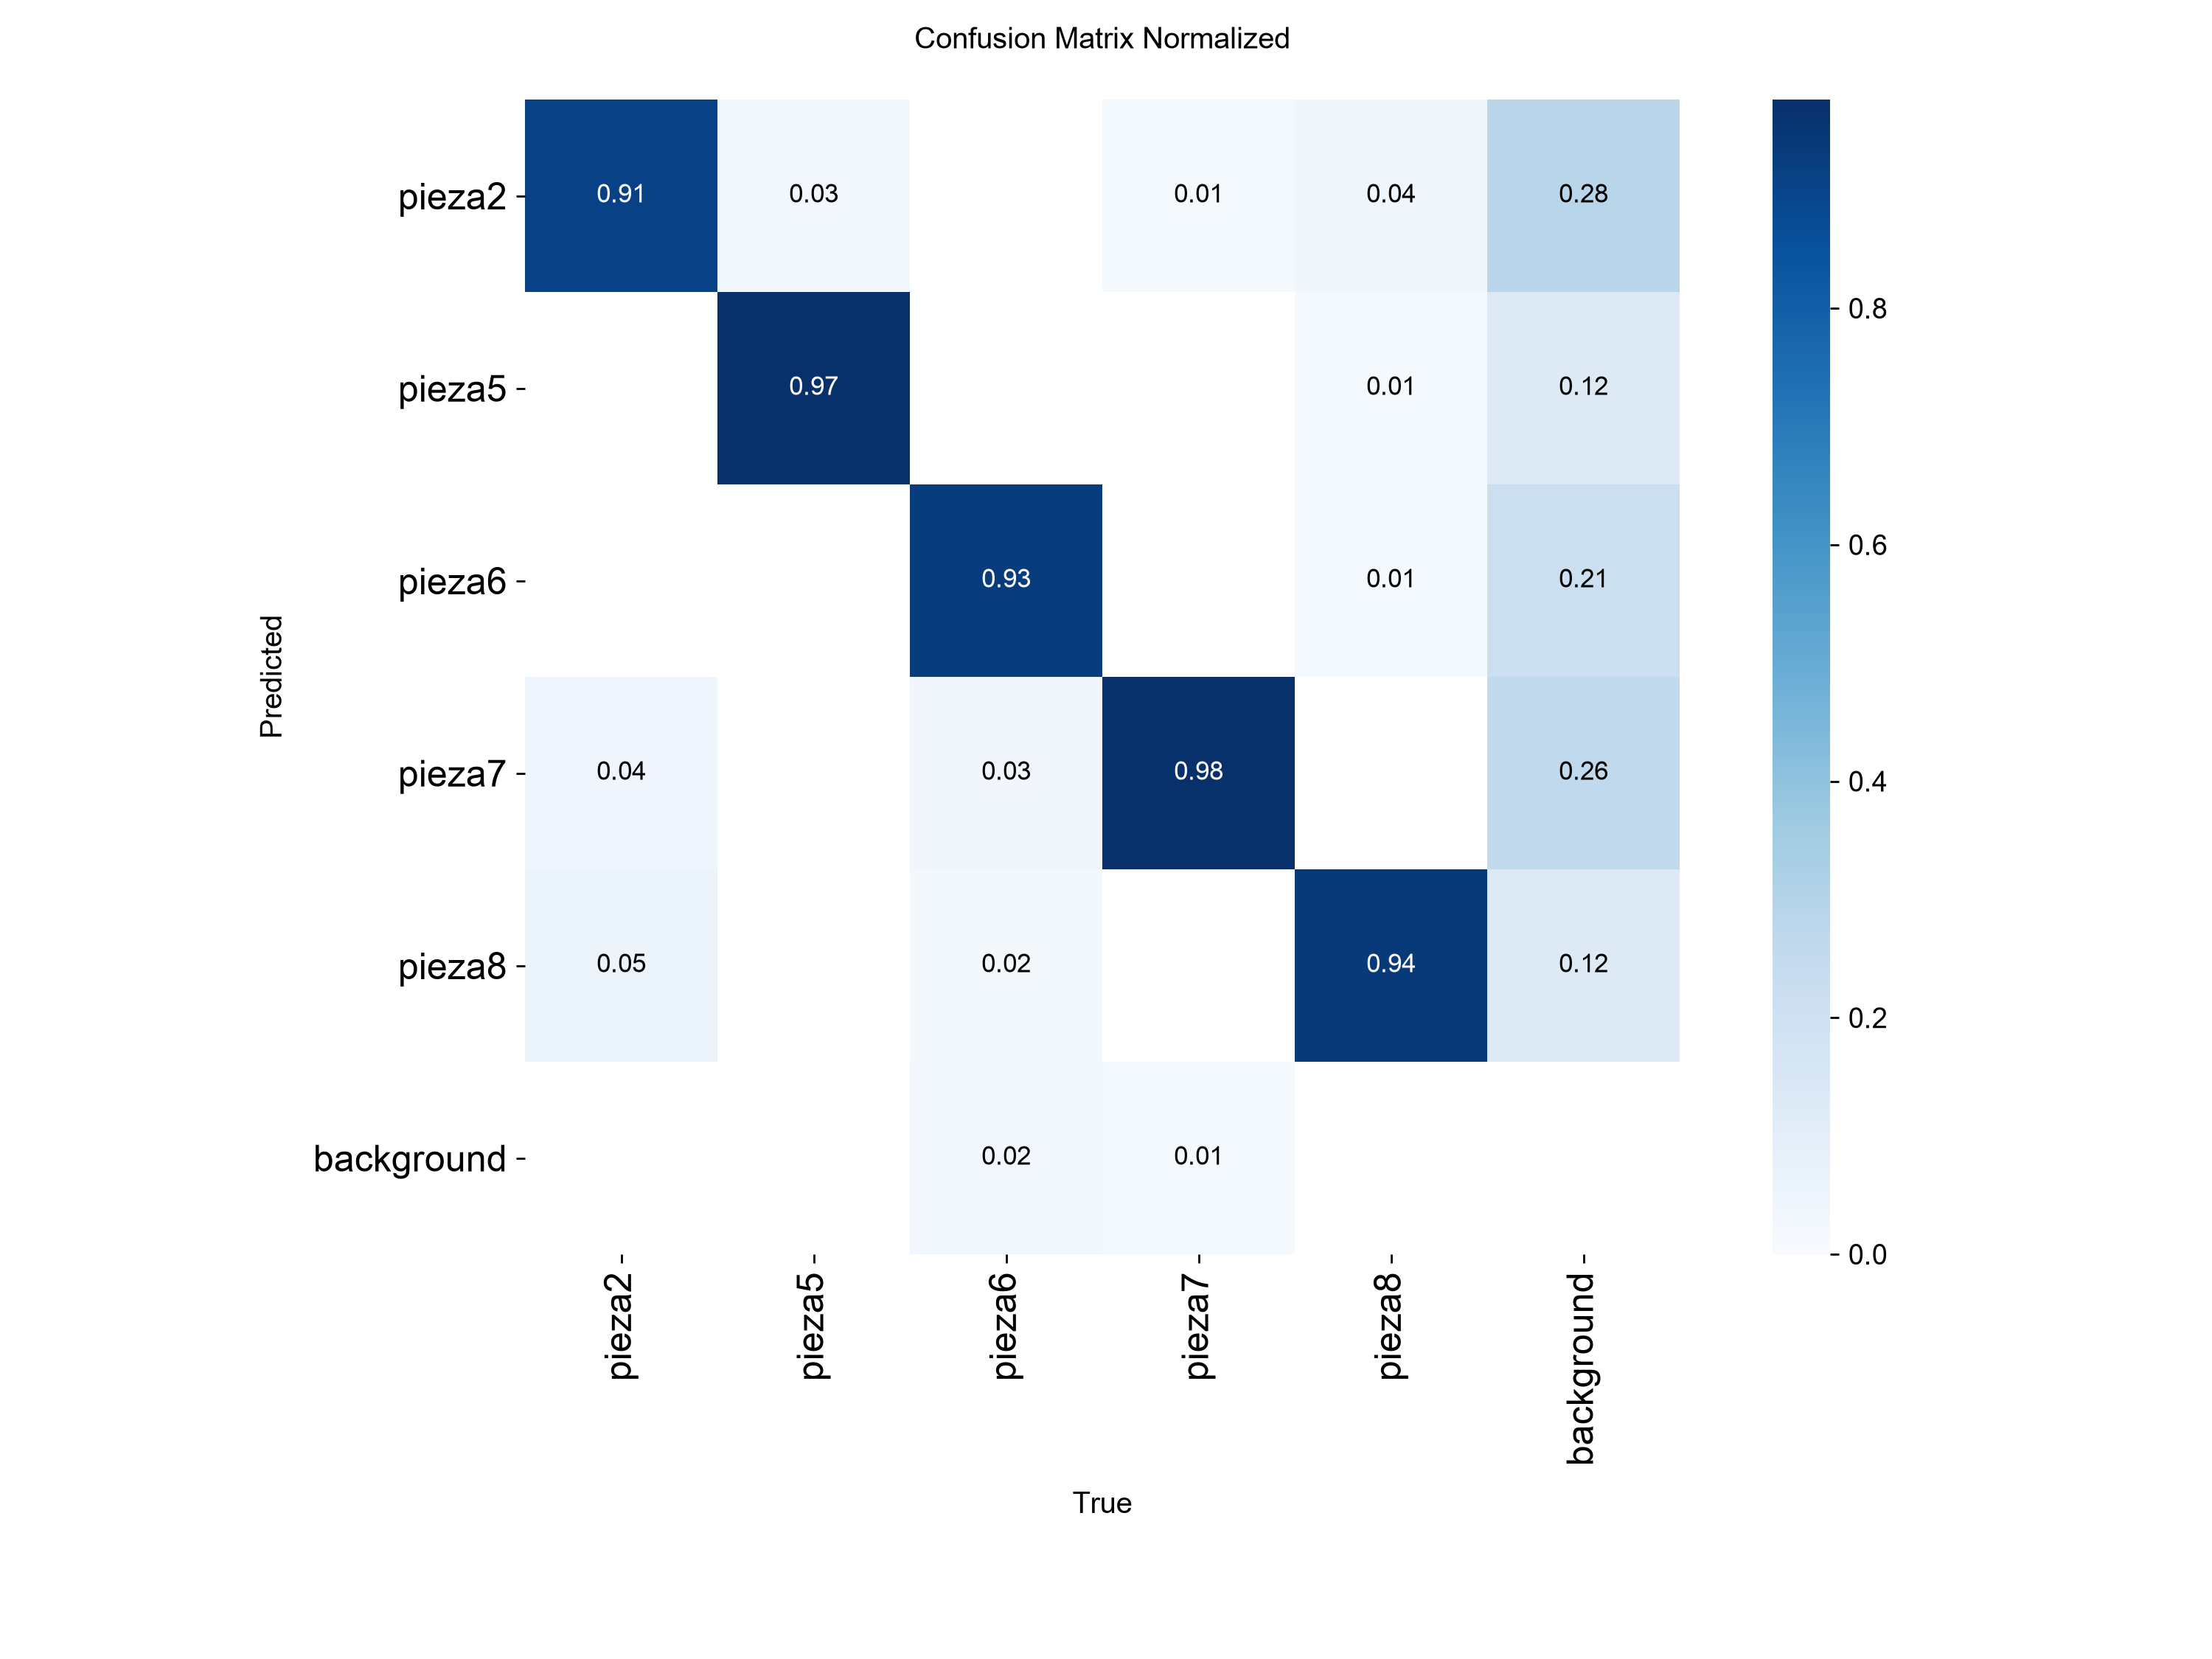
\includegraphics[width=0.80\textwidth,keepaspectratio]{figuras/fase5_matriz_confusion_seg.png}
    \caption{Matriz de confusión normalizada del modelo de segmentación sobre el conjunto de validación. Las columnas corresponden a la clase real y las filas a la clase predicha.}
    \label{fig:fase5_matriz_confusion}
    \par\small Fuente: elaboración propia, generada por Ultralytics durante la validación.
\end{figure}

Estas métricas se obtuvieron en computadora con el modelo antes de su cuantización y no con la cámara. Además, las imágenes de entrenamiento y validación provinieron de fotogramas de los mismos videos, por lo que ambos conjuntos pudieron contener escenas muy parecidas. En consecuencia, las métricas describieron el modelo, pero no constituyeron una medición de la clasificación en la cámara durante la operación; esta última no se cuantificó. El sistema utilizó la detección principalmente para localizar las piezas y estimar su orientación.


\subsection{Integración de la HUSKYLENS 2}

La HUSKYLENS 2 quedó integrada con la ESP32 mediante comunicación UART. La configuración utilizada correspondió a \texttt{HardwareSerial(1)}, con una velocidad de 115200 baudios y formato \texttt{SERIAL\_8N1}. El GPIO32 se utilizó como recepción desde la cámara y el GPIO33 como transmisión hacia esta.

La cámara se instaló en una posición fija sobre la estructura y orientada hacia la región de la banda utilizada para la detección de las piezas y la calibración geométrica. La disposición obtenida se muestra en la Figura~\ref{fig:fase5_ubicacion_camara}.

\begin{figure}[H]
    \centering
    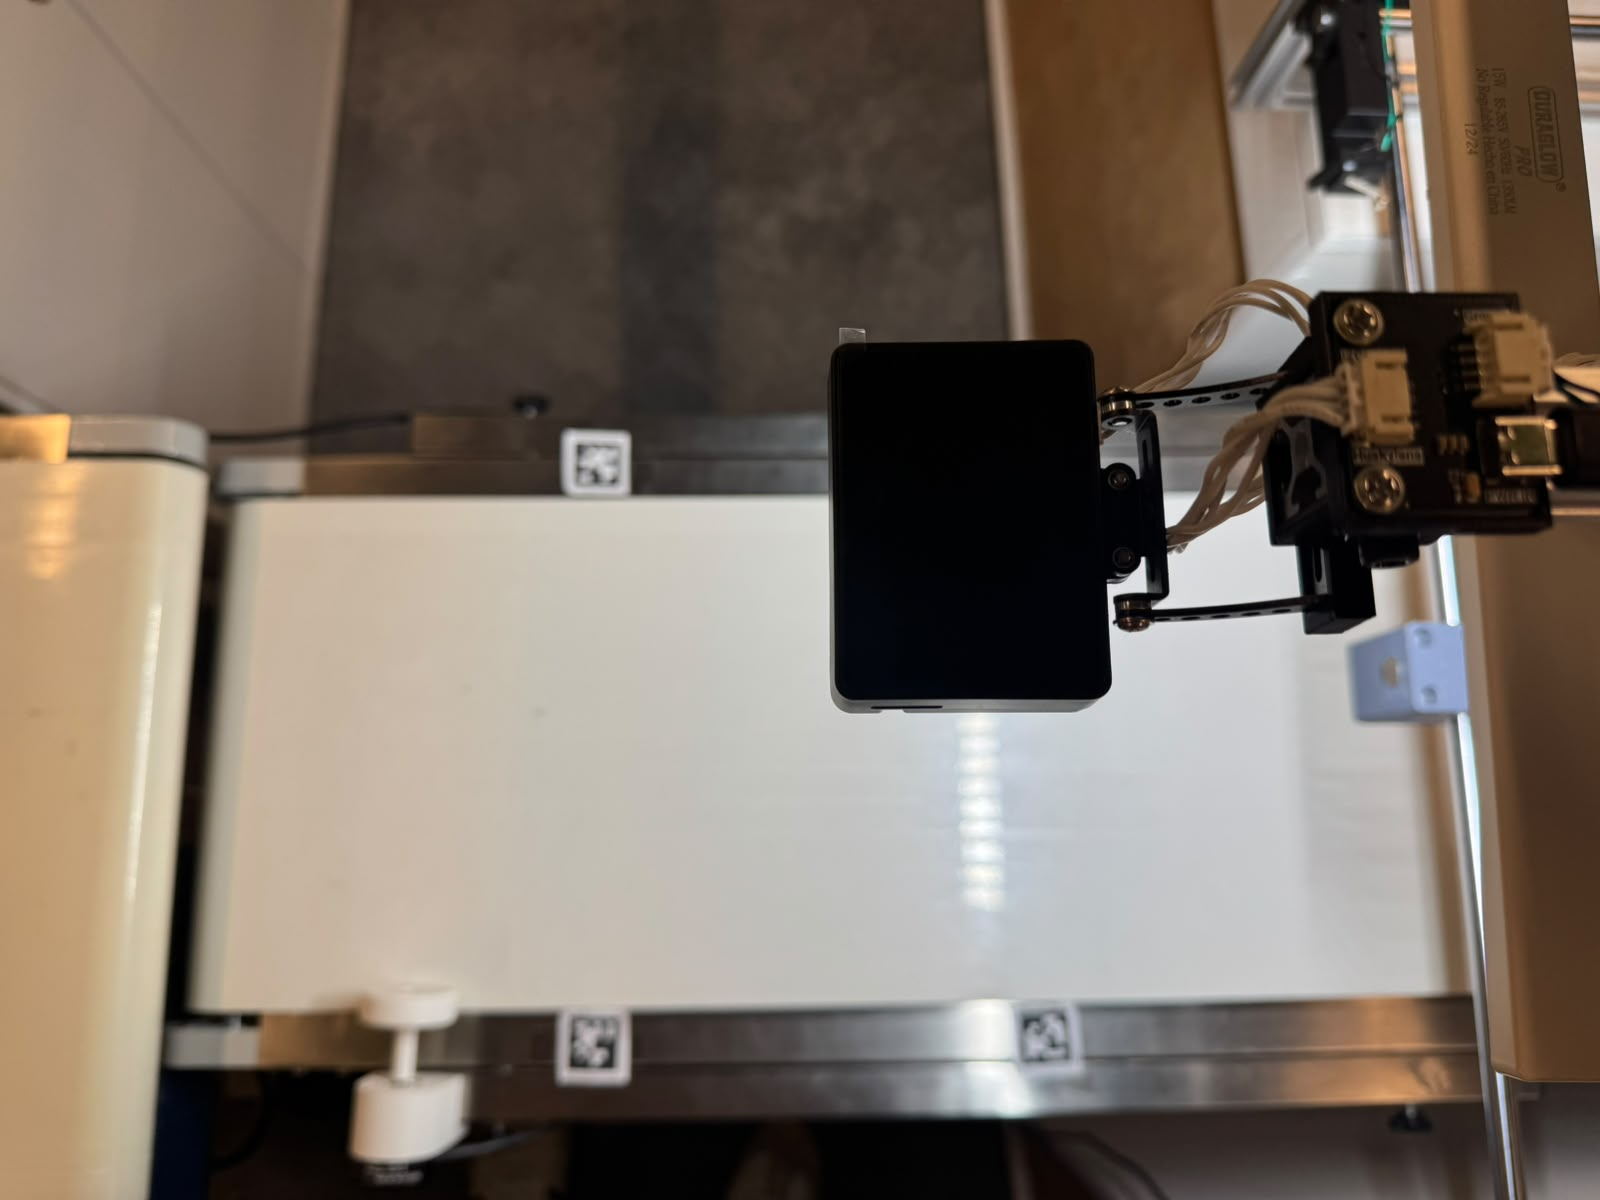
\includegraphics[
        width=0.72\textwidth,
        height=7.5cm,
        keepaspectratio
    ]{Imagenes de Documentacion/UbicaciondeCamara.jpeg}
    \caption{Ubicación de la HUSKYLENS 2 respecto de la banda transportadora durante la integración del sistema de visión.}
    \label{fig:fase5_ubicacion_camara}
    \par\small Fuente: elaboración propia.
\end{figure}

La administración de la cámara quedó centralizada en la función \texttt{procesarEstadoCamara()}, ejecutada periódicamente desde la tarea \texttt{tareaCamara()}.

La implementación permitió representar el estado de la cámara mediante la secuencia:

\[
\begin{aligned}
\texttt{OFFLINE}
&\rightarrow
\texttt{CONECTANDO}
\rightarrow
\texttt{STANDBY}
\rightarrow
\texttt{ABRIENDO\_TAGS}
\rightarrow
\texttt{CALIBRANDO}
\\[2mm]
&\rightarrow
\texttt{CALCULANDO}
\rightarrow
\texttt{ABRIENDO\_MODELO}
\rightarrow
\texttt{LISTA}.
\end{aligned}
\]

La secuencia permitió utilizar inicialmente el algoritmo de AprilTags durante la calibración y posteriormente abrir el modelo personalizado utilizado para la detección de piezas.

El modelo personalizado quedó configurado con:

\[
\texttt{CUSTOM\_MODEL\_INDEX}=1,
\]

correspondiente a \texttt{ALGORITHM\_CUSTOM\_BEGIN + 1}, es decir, al algoritmo 129 de la cámara. Aunque el modelo es de segmentación, la interfaz UART de la cámara entregó para cada detección únicamente el nombre de la clase, el centro y el ancho y alto de la caja delimitadora, sin la máscara.

La función \texttt{getResult()} se utilizó durante la comunicación con la cámara para obtener respuestas y resultados del algoritmo activo. Una respuesta válida sin objetos permitió diferenciar la disponibilidad de la comunicación de la existencia de una detección.

La gestión de la cámara se ejecutó mediante una tarea independiente de FreeRTOS creada mediante \texttt{xTaskCreatePinnedToCore()}. Esto permitió mantener la adquisición visual separada de las funciones asociadas con el mando, la pantalla OLED, los servomotores y el enlace de control entre la Portenta H7 y la ESP32.

La integración mediante UART sustituyó la configuración inicial de la cámara mediante I2C. En la configuración posterior, la cámara dispuso de un enlace UART independiente, la pantalla OLED continuó conectada mediante I2C a la ESP32 y la comunicación entre la ESP32 y la Portenta H7 se realizó mediante UART sobre RS485.


\subsection{Calibración geométrica del plano de trabajo}

La calibración visual utilizó cuatro AprilTags identificados como 0, 1, 2 y 3. La disposición física de los marcadores sobre la banda se muestra en la Figura~\ref{fig:fase5_apriltags}.

\begin{figure}[H]
    \centering
    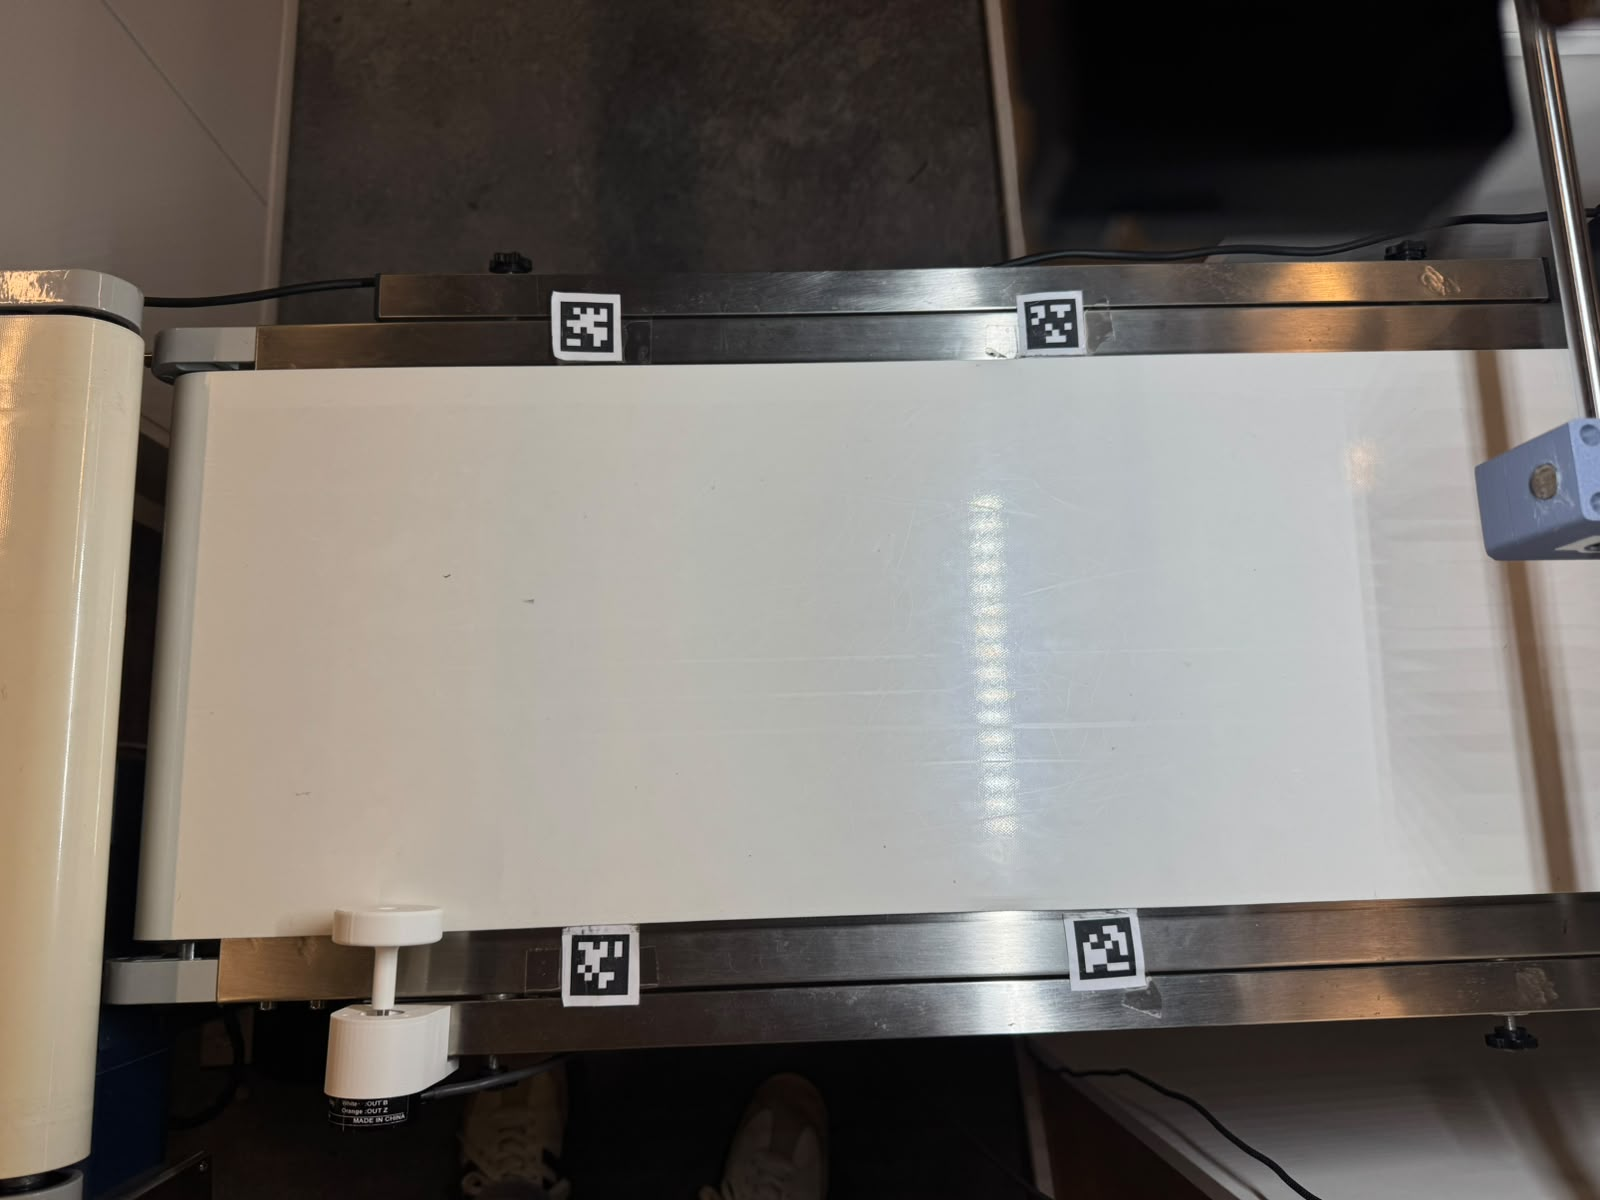
\includegraphics[
        width=0.75\textwidth,
        height=7.5cm,
        keepaspectratio
    ]{Imagenes de Documentacion/AprilTagsenBanda.jpeg}
    \caption{Disposición de los cuatro marcadores AprilTag utilizados para la calibración geométrica del plano de trabajo.}
    \label{fig:fase5_apriltags}
    \par\small Fuente: elaboración propia.
\end{figure}

Para cada marcador se utilizaron 25 observaciones de su centro antes de calcular la transformación. La geometría configurada utilizó un ancho útil de banda de 292~mm, un ancho total de 412~mm y una separación longitudinal de 255~mm entre las filas de marcadores.

Inicialmente, el firmware se configuró con una separación de 382~mm entre filas. Al comparar las trayectorias registradas de las piezas con el avance medido por el encoder, el desplazamiento longitudinal calculado por la cámara resultó entre 1,42 y 1,55 veces mayor que el de la banda. Además, una misma pieza medía entre 75 y 78 píxeles de largo en X y en Y, pero la homografía le asignaba 0,69~mm/píxel en X y 0,99~mm/píxel en Y. La separación se corrigió a 255~mm, valor que coincidió con la distancia física entre las filas de marcadores. No se registró una nueva comparación entre el recorrido medido por la cámara y el del encoder después de la corrección. En las mismas trayectorias se comprobó que la coordenada Y de la homografía crecía en el sentido de avance de la banda, lo que corrigió también el signo utilizado para transformarla al sistema del brazo.

Las coordenadas de referencia utilizadas por el firmware se resumieron en el Cuadro~\ref{tab:fase5_tags}.

\begin{table}[H]
    \centering
    \caption{Coordenadas de referencia utilizadas para los cuatro AprilTags.}
    \label{tab:fase5_tags}
    \begin{tabular}{crr}
        \hline
        Identificador & $X_c$ (mm) & $Y_c$ (mm) \\
        \hline
        0 & $-176$ & $-127{,}5$ \\
        1 & $176$ & $-127{,}5$ \\
        2 & $176$ & $127{,}5$ \\
        3 & $-176$ & $127{,}5$ \\
        \hline
    \end{tabular}

    \par\small\raggedright Fuente: elaboración propia a partir de la configuración utilizada por el sistema de visión.
\end{table}

La secuencia produjo una matriz de homografía válida para convertir los centros detectados en píxeles a coordenadas métricas dentro del plano configurado.

La transformación se utilizó posteriormente para generar los objetivos de posicionamiento del brazo y para descartar detecciones ubicadas fuera del área configurada como válida.

La matriz numérica correspondiente a una calibración final y el error obtenido sobre puntos independientes no se registraron. Por esta razón, la transformación se presentó como funcional, pero no como una medición de exactitud geométrica.


\subsection{Integración del encoder de la banda transportadora}

El encoder incremental quedó instalado junto a la banda transportadora para obtener información de desplazamiento durante la operación automática. Su instalación física se muestra en la Figura~\ref{fig:fase5_encoder}.

\begin{figure}[H]
    \centering
    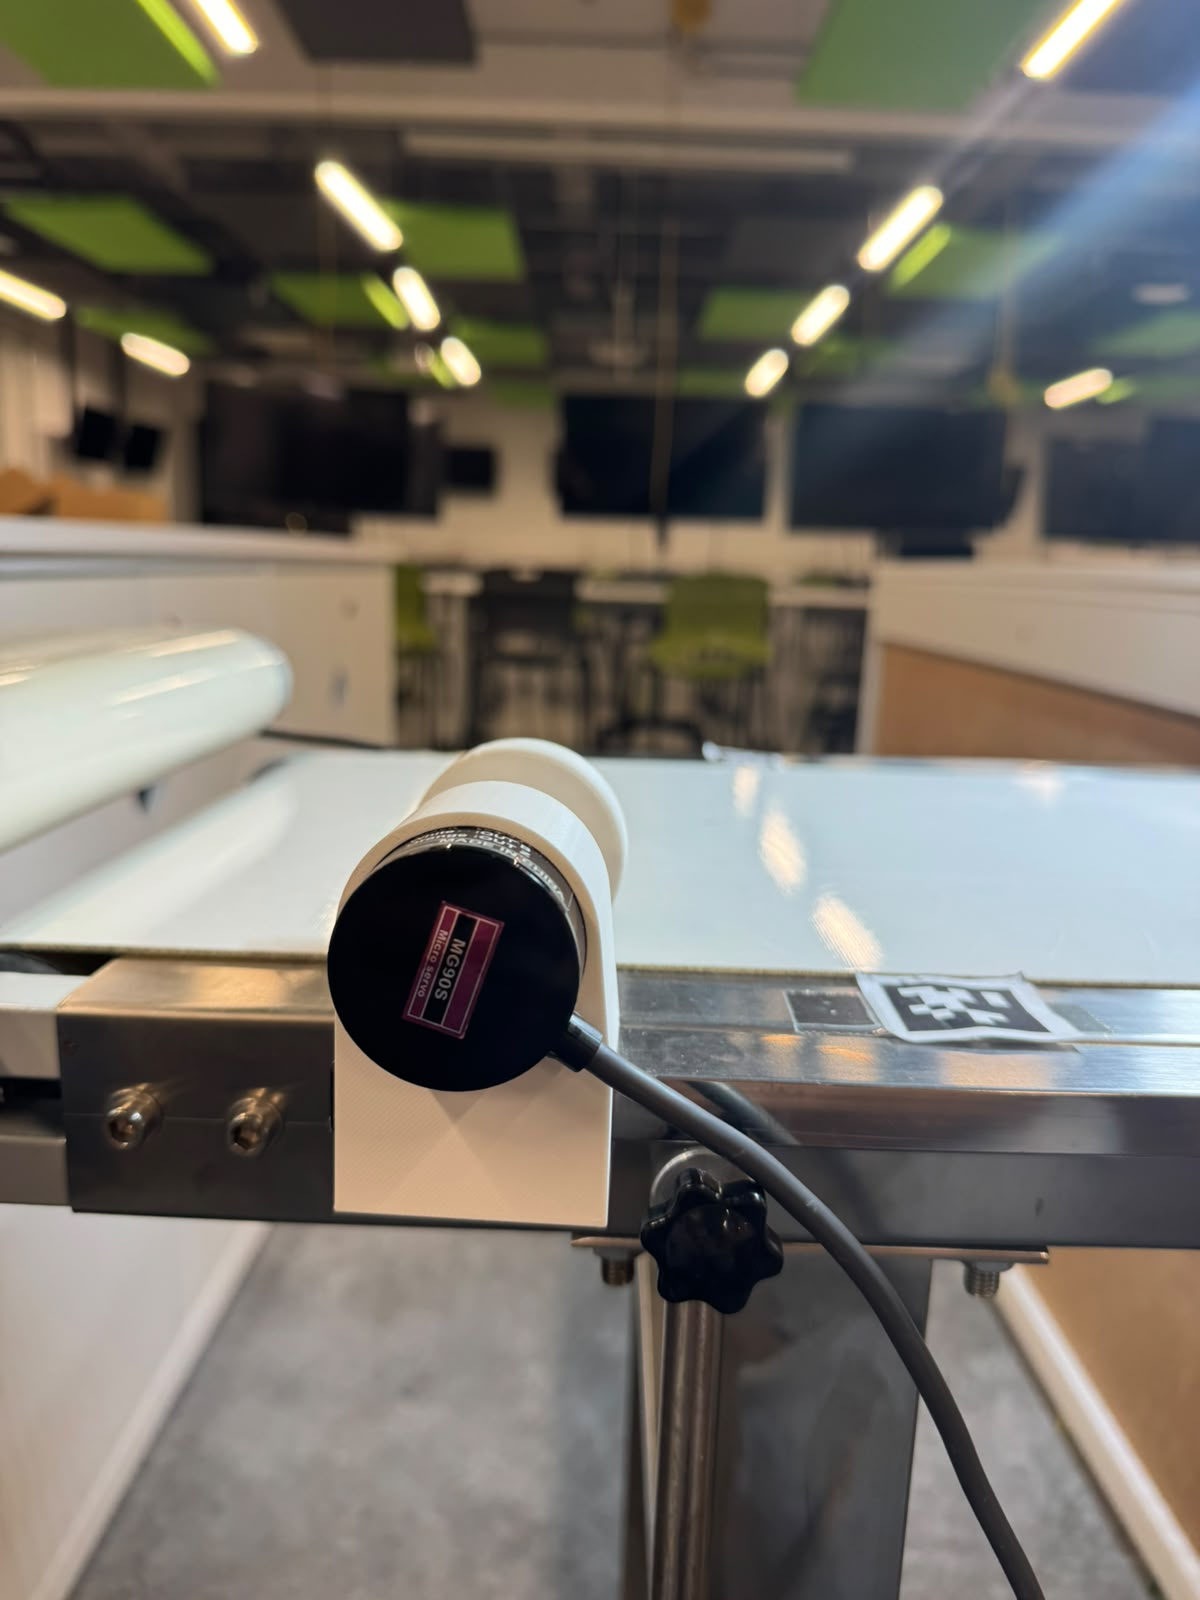
\includegraphics[
        width=0.60\textwidth,
        height=7.0cm,
        keepaspectratio
    ]{Imagenes de Documentacion/Encoder.jpeg}
    \caption{Encoder incremental instalado para la medición del desplazamiento de la banda transportadora.}
    \label{fig:fase5_encoder}
    \par\small Fuente: elaboración propia.
\end{figure}

El encoder Omron E6B2-CWZ6C quedó integrado a la interfaz de encoder de Machine Control y fue procesado directamente por la Portenta H7.

La configuración utilizó las entradas A0, B0 y Z0 del encoder 0. El firmware empleó 1024 pulsos por revolución y decodificación X2, equivalente a 2048 cuentas por revolución.

Con una rueda configurada de 49~mm de diámetro y una relación 1:1 se obtuvo una escala utilizada por el firmware de aproximadamente:

\[
0{,}0752~\text{mm/cuenta}.
\]

La función \texttt{actualizarEncoderBanda()} proporcionó al sistema las variables utilizadas para representar el conteo, sentido y desplazamiento de la banda.

La información obtenida se incorporó al protocolo entre la Portenta y la ESP32 y posteriormente se utilizó durante el modo automático para actualizar la posición longitudinal estimada de las piezas.

La escala indicada correspondió a la configuración utilizada por el firmware. No se dispuso todavía de una comparación con un patrón externo de longitud que permitiera reportar su error metrológico.


\subsection{Sincronización y modo automático}

La integración del sistema de visión con el movimiento se comprobó inicialmente con la banda detenida, mediante el modo automático que solo desplaza X y Y.

En cinco pruebas funcionales, el brazo se desplazó hasta la ubicación correspondiente de la pieza en los cinco casos según el criterio funcional utilizado durante esta etapa.

No se realizó la recogida de la pieza durante estas cinco pruebas y no se registró un error de posición en milímetros.

\begin{table}[H]
    \centering
    \caption{Resultado de las pruebas funcionales de posicionamiento con la banda detenida.}
    \label{tab:fase5_prueba_estatica}
    \begin{tabular}{p{0.61\textwidth}p{0.25\textwidth}}
        \hline
        Indicador & Resultado \\
        \hline
        Pruebas realizadas & 5 \\
        Desplazamientos hasta la ubicación de la pieza & 5 \\
        Casos sin coincidencia funcional reportada & 0 \\
        Proporción observada en la serie & 5/5 (100\%) \\
        Recogida de piezas & No realizada en esta subetapa \\
        Error de posición en milímetros & No documentado \\
        \hline
    \end{tabular}

    \par\small\raggedright Fuente: elaboración propia a partir de los resultados funcionales registrados durante la etapa de posicionamiento estático.
\end{table}

Posteriormente se integró la información del encoder al flujo automático. El modo automático con la banda en movimiento incorporó la cuenta del encoder asociada con cada objetivo, la orientación automática de la garra y la secuencia completa de captura y entrega descrita en la metodología: aceptación del objetivo, preposicionamiento en la X de la pieza y en la estación $Y=0$, descenso de Z a la altura de espera, predicción del contacto, descenso final, confirmación del final de carrera inferior, cierre y confirmación de la pinza, retirada de Z, traslado al punto de entrega, descenso, apertura de la pinza y regreso a la altura segura.

En la primera versión de este modo, la transformación entre la cámara y el brazo utilizaba una distancia de 845~mm entre el centro de la homografía y la estación de captura, junto con el signo invertido de Y y la escala longitudinal inflada descrita en la Sección~\ref{sec:resultados_fase5}. Estos tres errores se compensaban entre sí solo para las piezas observadas cerca de $Y=-170$~mm, por lo que el error de captura dependía de la posición en que la cámara veía la pieza. Con 22 agarres manuales exitosos registrados en el modo de enseñanza, el error de posición de la pieza en el instante de contacto, calculado con el modelo anterior, fue de $-69\pm103$~mm; con el modelo corregido, de $-1\pm24$~mm. Estos agarres se realizaron con velocidades de banda de 70 a 95~mm/s.

Los ensayos posteriores en la maqueta con una pieza vertical de 48~mm, marcada en su centro, mostraron que con 565~mm la pinza cerraba unos 14~mm después del centro, por lo que la distancia se fijó en 551~mm. Con ese valor, las piezas horizontales descendían unos 20~mm antes de lo necesario y el dedo de aguas arriba caía delante de la pieza, lo que motivó el retraso de $40\,\lvert\cos\theta\rvert$~mm. El Cuadro~\ref{tab:fase5_modelo_posicion} compara los parámetros de ambas versiones.

\begin{table}[H]
    \centering
    \caption{Parámetros del modelo de posición de la pieza antes y después de la corrección.}
    \label{tab:fase5_modelo_posicion}
    \begin{tabular}{p{0.36\textwidth}p{0.24\textwidth}p{0.28\textwidth}}
        \hline
        Parámetro & Versión inicial & Versión final (V4) \\
        \hline
        Separación entre filas de AprilTags & 382~mm & 255~mm \\
        Signo de Y cámara--brazo & $-1$ & $+1$ \\
        Distancia homografía--captura & 845~mm & 551~mm \\
        Transformación en X & $X_b=-X_c-5$~mm & $X_b=-X_c-5$~mm \\
        Retraso por orientación & No aplicado & $40\,\lvert\cos\theta\rvert$~mm \\
        Tiempo de la orden de cierre al contacto & 608~ms & 300~ms \\
        Error de posición al contacto (22 agarres) & $-69\pm103$~mm & $-1\pm24$~mm \\
        \hline
    \end{tabular}
    \par\small\raggedright Fuente: elaboración propia a partir de la configuración del firmware y de los registros del modo de enseñanza.
\end{table}

Los registros electrónicos del modo automático mostraron secuencias que alcanzaron la orden de cierre, la confirmación de la pinza y la finalización del ciclo. Sin embargo, el final de carrera inferior confirmó únicamente la altura de Z y no la presencia de la pieza en la garra. Por esta razón, el firmware registró cada ciclo terminado como entregado sin agarre verificado, y el éxito se evaluó mediante la observación directa de 120 intentos, cuyos resultados se presentan en la Sección~\ref{sec:resultados_fase6}.

% ============================================================
% FASE 6: VALIDACIÓN EXPERIMENTAL DEL AGARRE
% ============================================================

\section{Fase 6. Validación experimental}
\label{sec:resultados_fase6}

\subsection{Registro de las pruebas de recogida y entrega}

Se registraron 120 intentos del ciclo automático con la banda en movimiento, ejecutados con el firmware V4 y distribuidos en dos condiciones identificadas en el registro experimental como 35~\% y 25~\% de velocidad de la banda transportadora. En cada condición se evaluaron 30 intentos con la pieza 6 y 30 con la pieza 7, para un total de 60 ensayos por condición. Cada intento se consignó mediante un identificador de prueba, el tipo de pieza, una respuesta binaria (\textit{Sí} o \textit{No}) y una observación sobre la orientación de la pieza. Un intento se registró como exitoso cuando el brazo recogió la pieza y la depositó en el punto de entrega.

Las orientaciones consignadas fueron vertical, horizontal y diagonal. Se calculó la proporción de éxito como el cociente entre los intentos marcados como \textit{Sí} y el total de intentos del grupo, expresado en porcentaje:

\begin{equation}
    \text{Éxito}~(\%) = \frac{N_{\text{ciclos exitosos}}}{N_{\text{intentos registrados}}}\times 100.
    \label{eq:fase6_tasa_exito}
\end{equation}

Los porcentajes de velocidad identificaron las consignas utilizadas durante los ensayos. No se conservaron los registros del firmware de estas sesiones, por lo que no se dispuso de la velocidad lineal de la banda en mm/s para cada consigna. En consecuencia, no se asumió una equivalencia entre las consignas porcentuales y velocidades físicas específicas.

\subsection{Tasa de éxito según velocidad y tipo de pieza}

El Cuadro~\ref{tab:fase6_resumen_agarre} presenta las frecuencias registradas y las tasas de éxito calculadas. En total se documentaron 74 ciclos exitosos y 46 fallidos, correspondientes a una tasa de éxito global de 61,7~\%.

\begin{table}[H]
    \centering
    \caption{Resultados de las pruebas de recogida y entrega por condición de velocidad y tipo de pieza.}
    \label{tab:fase6_resumen_agarre}
    \begin{tabular}{l l r r r r}
        \hline
        Velocidad & Pieza & Intentos & Exitosos & Fallidos & Éxito (\%) \\
        \hline
        35\% & Pieza 6 & 30 & 12 & 18 & 40,0 \\
             & Pieza 7 & 30 & 18 & 12 & 60,0 \\
             & Total   & 60 & 30 & 30 & 50,0 \\
        \hline
        25\% & Pieza 6 & 30 & 17 & 13 & 56,7 \\
             & Pieza 7 & 30 & 27 & 3  & 90,0 \\
             & Total   & 60 & 44 & 16 & 73,3 \\
        \hline
        Ambos & Total & 120 & 74 & 46 & 61,7 \\
        \hline
    \end{tabular}
    \par\small\raggedright Fuente: elaboración propia a partir de \textit{Pruebas\_Agarre\_Brazo.xlsx}, hojas \textit{Vel 35\%}, \textit{Vel 25\%} y \textit{Resumen}.
\end{table}

La condición del 25~\% presentó 44 ciclos exitosos de 60 intentos (73,3~\%), mientras que la del 35~\% registró 30 de 60 (50,0~\%). La diferencia observada entre las tasas fue de 23,3 puntos porcentuales a favor de la condición del 25~\%. Por tipo de pieza, la pieza 7 alcanzó 90,0~\% en la condición del 25~\% y 60,0~\% en la del 35~\%, mientras que la pieza 6 alcanzó 56,7~\% y 40,0~\%, respectivamente.

La Figura~\ref{fig:fase6_exito_pieza_velocidad} representa estas proporciones junto con el número de ciclos exitosos y el total de intentos correspondiente a cada grupo.

\begin{figure}[H]
    \centering
    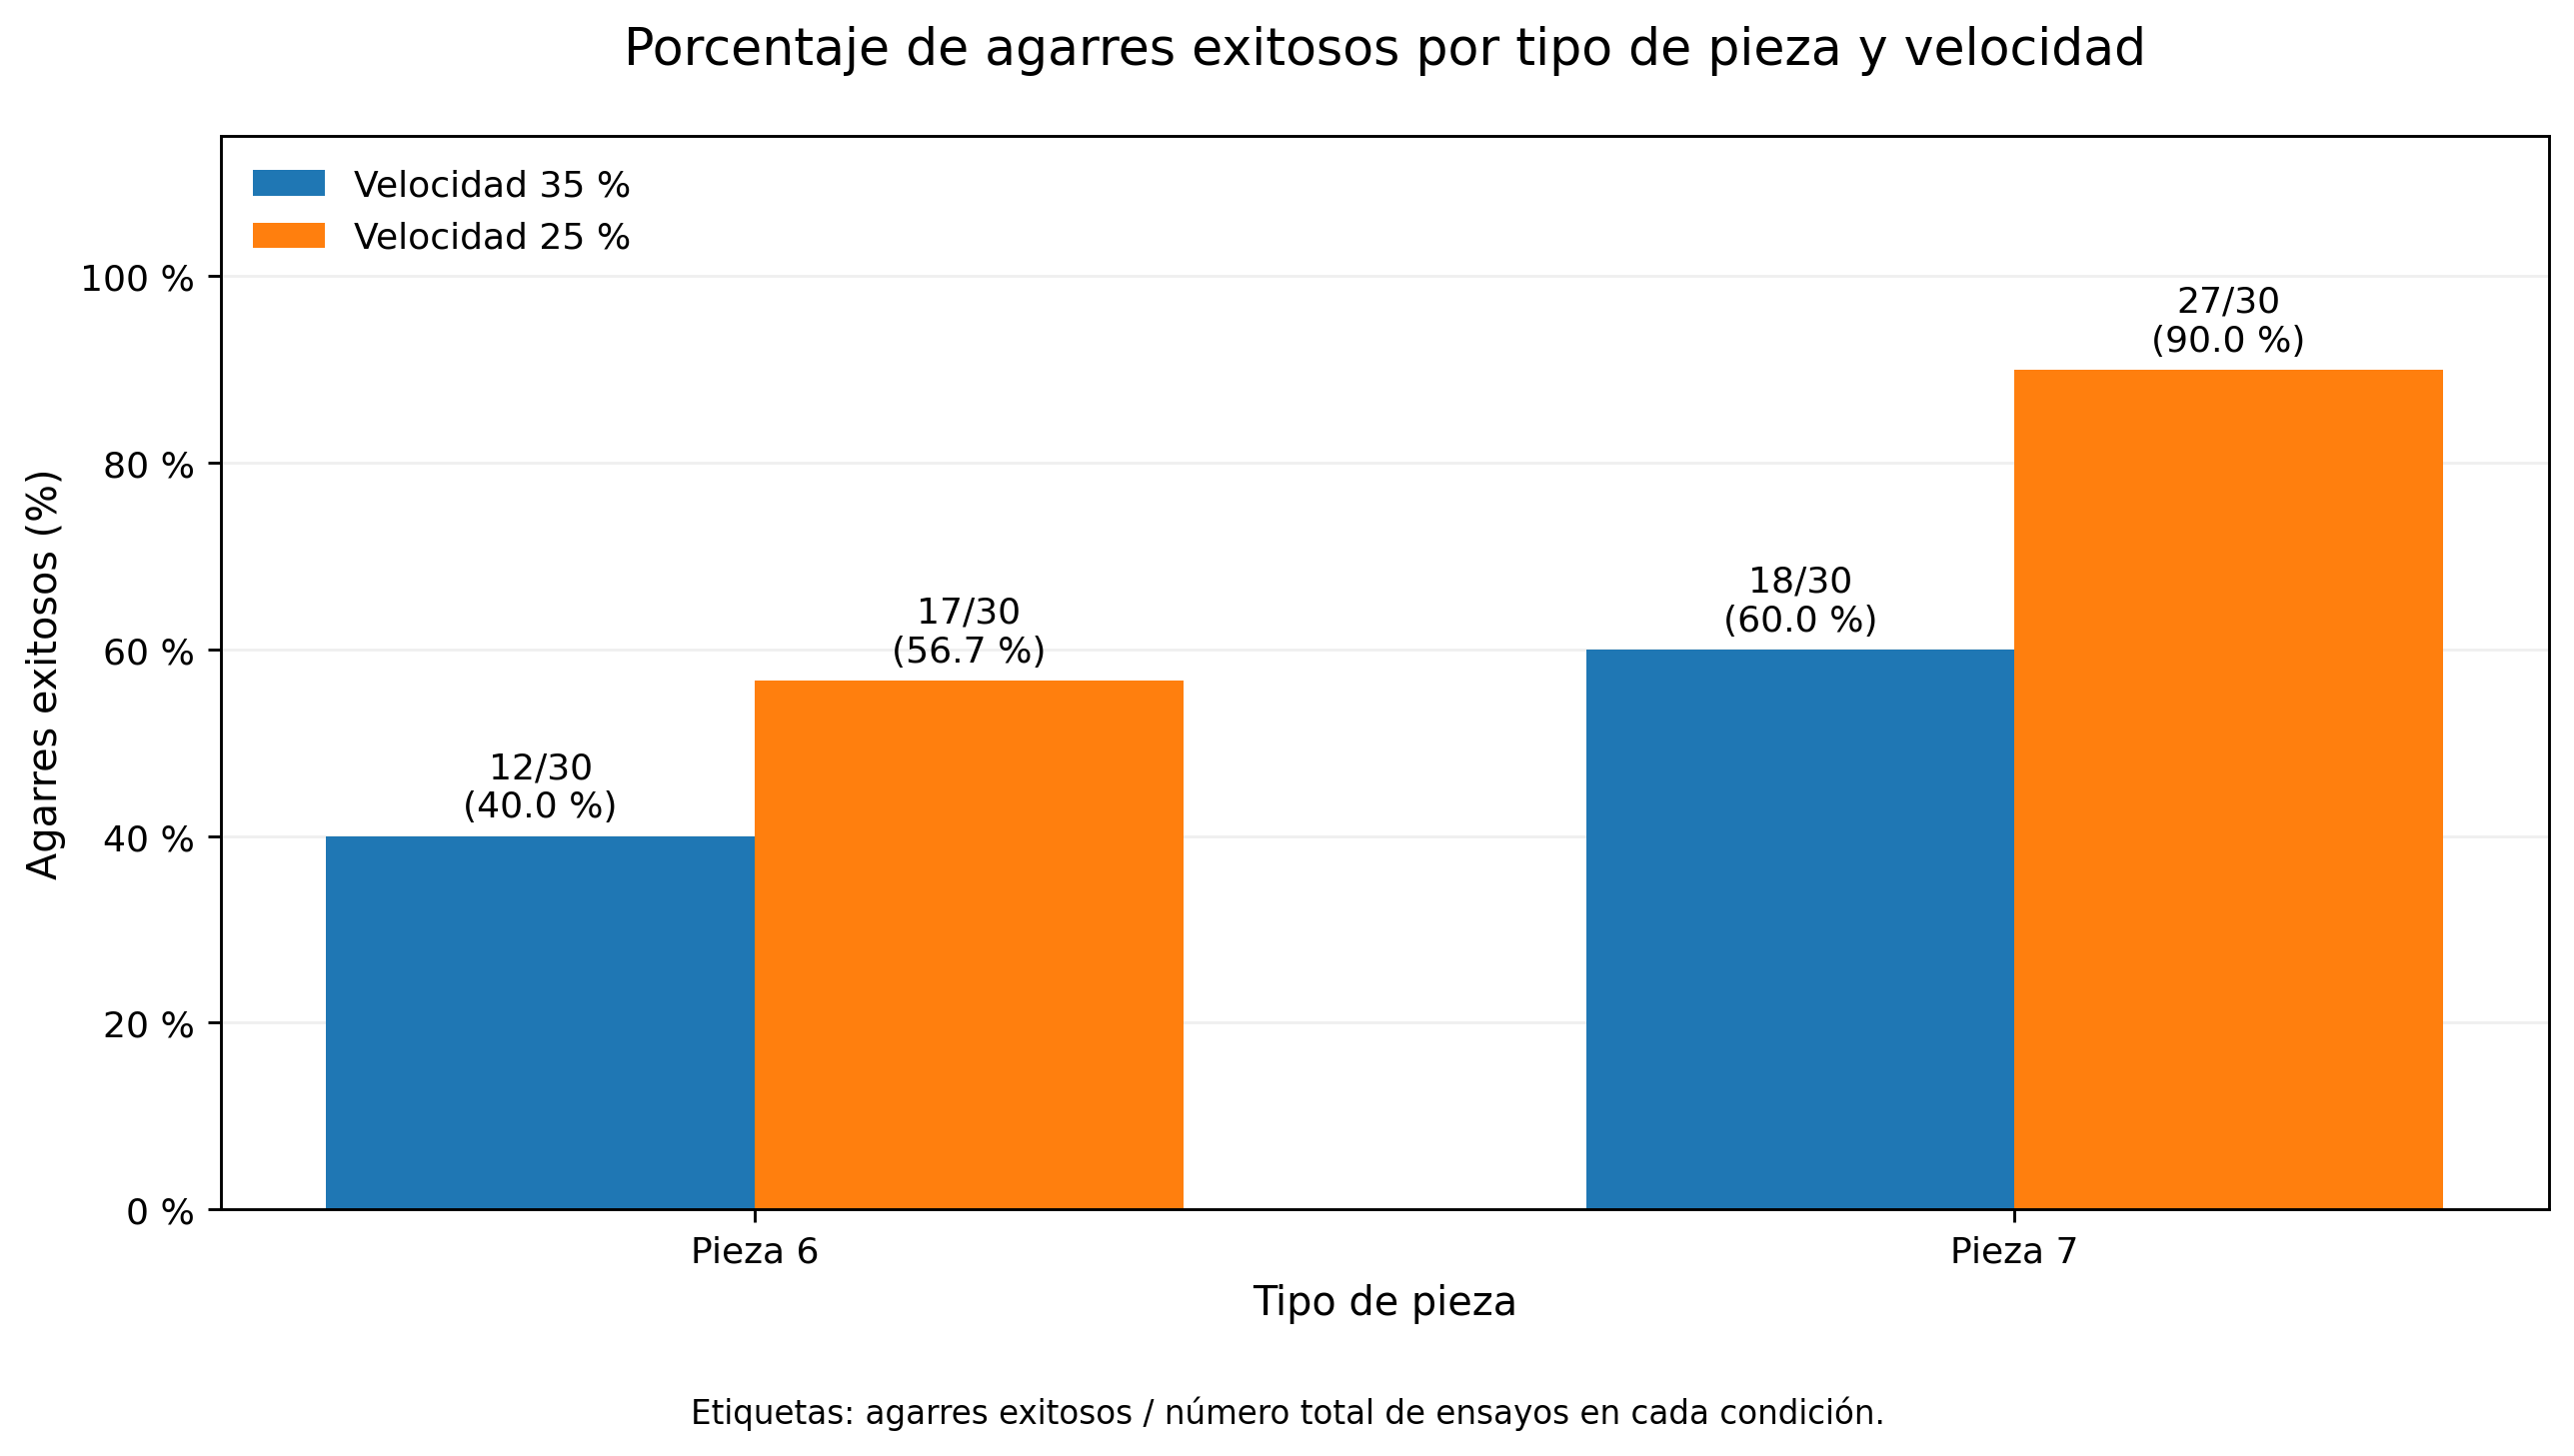
\includegraphics[width=0.88\textwidth,keepaspectratio]{figuras/fase6_exito_pieza_velocidad.png}
    \caption{Porcentaje de ciclos exitosos por tipo de pieza y condición de velocidad. Los valores entre paréntesis indican ciclos exitosos e intentos totales.}
    \label{fig:fase6_exito_pieza_velocidad}
    \par\small Fuente: elaboración propia a partir del registro experimental de recogida y entrega.
\end{figure}

\subsection{Resultados según la orientación de las piezas}

El registro permitió desagregar los ensayos de cada pieza en tres orientaciones. El número de intentos no fue uniforme entre orientaciones: en las dos condiciones de velocidad se realizaron, en conjunto, 32 pruebas verticales, 31 horizontales y 57 diagonales. El Cuadro~\ref{tab:fase6_orientacion_detalle} conserva esta distinción y presenta los resultados específicos de cada combinación.

\begin{table}[H]
    \centering
    \caption{Resultados de recogida y entrega por velocidad, tipo de pieza y orientación.}
    \label{tab:fase6_orientacion_detalle}
    \begin{tabular}{l l l r r r}
        \hline
        Velocidad & Pieza & Orientación & Intentos & Exitosos & Éxito (\%) \\
        \hline
        35\% & Pieza 6 & Vertical   & 8  & 7  & 87,5 \\
             &         & Horizontal & 7  & 2  & 28,6 \\
             &         & Diagonal   & 15 & 3  & 20,0 \\
             & Pieza 7 & Vertical   & 8  & 8  & 100,0 \\
             &         & Horizontal & 8  & 5  & 62,5 \\
             &         & Diagonal   & 14 & 5  & 35,7 \\
        \hline
        25\% & Pieza 6 & Vertical   & 8  & 6  & 75,0 \\
             &         & Horizontal & 8  & 1  & 12,5 \\
             &         & Diagonal   & 14 & 10 & 71,4 \\
             & Pieza 7 & Vertical   & 8  & 8  & 100,0 \\
             &         & Horizontal & 8  & 6  & 75,0 \\
             &         & Diagonal   & 14 & 13 & 92,9 \\
        \hline
    \end{tabular}
    \par\small\raggedright Fuente: elaboración propia a partir de las observaciones registradas en ambas hojas de ensayos.
\end{table}

Al agrupar las dos piezas, los ensayos verticales registraron 29 éxitos de 32 intentos (90,6~\%); los horizontales, 14 de 31 (45,2~\%); y los diagonales, 31 de 57 (54,4~\%). La Figura~\ref{fig:fase6_exito_orientacion} muestra estas tasas separadas por condición de velocidad, sin suponer que el número desigual de pruebas por orientación representa una distribución proporcional del proceso productivo.

\begin{figure}[H]
    \centering
    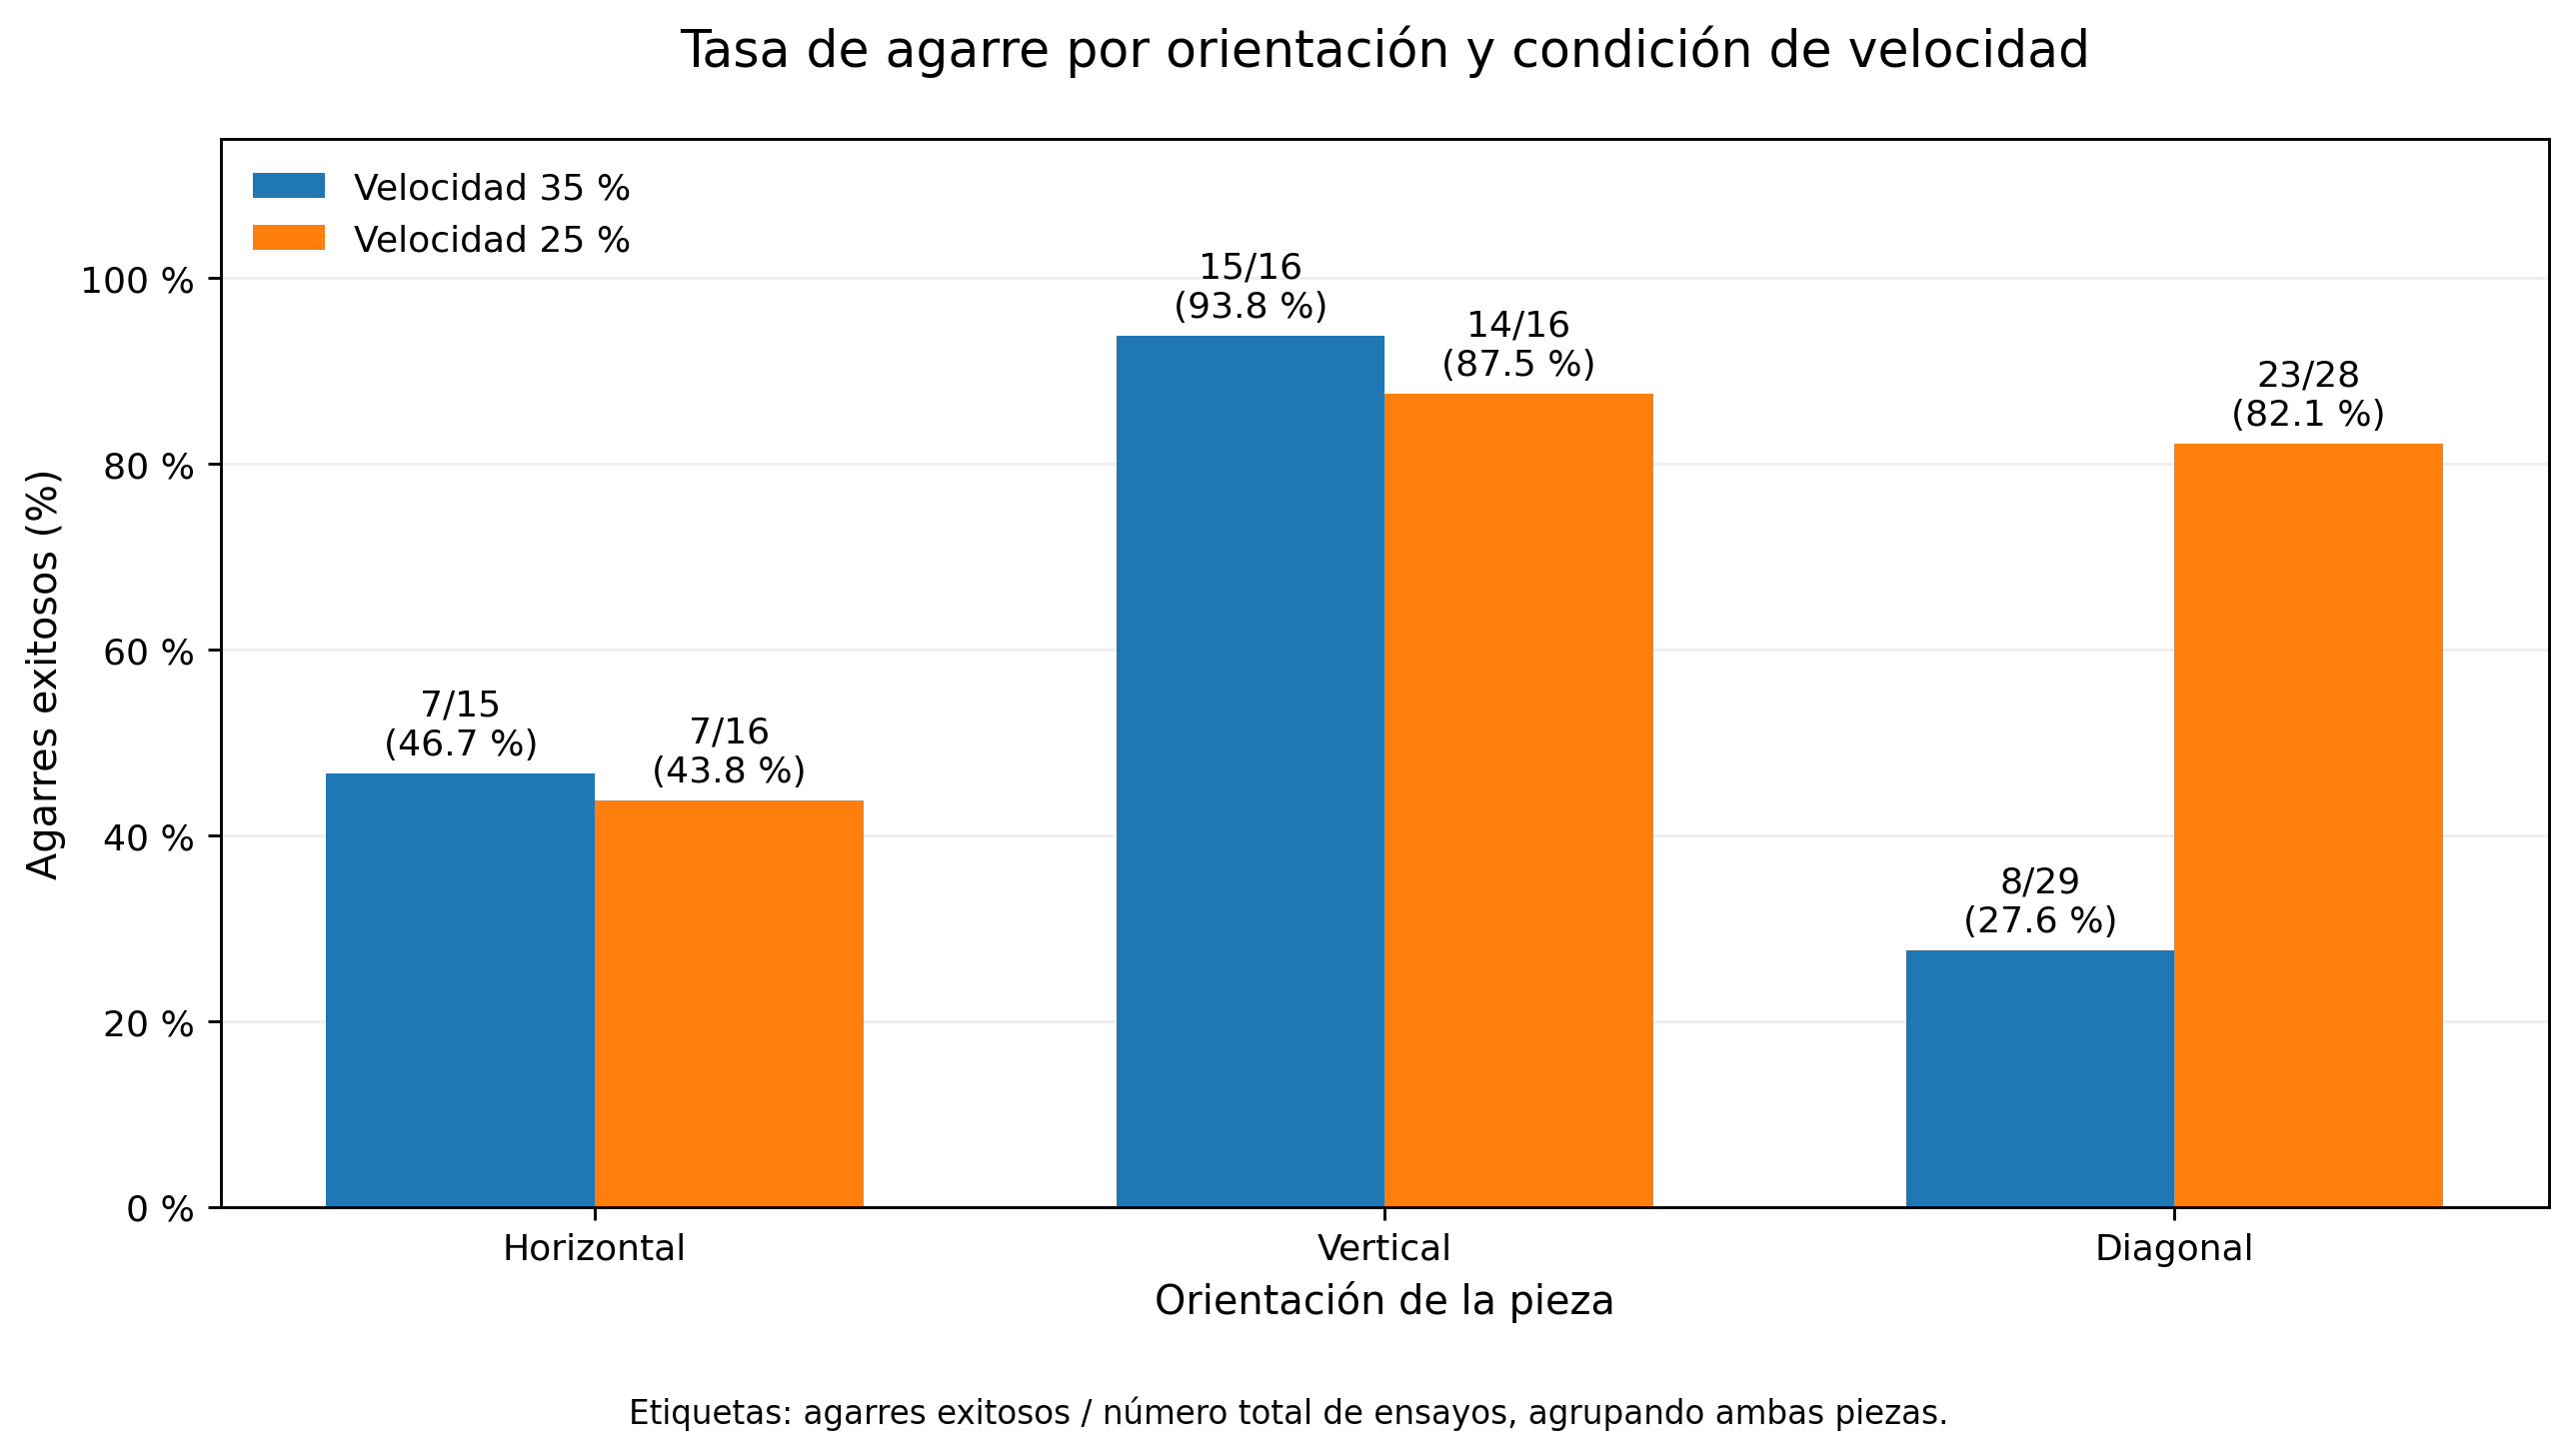
\includegraphics[width=0.88\textwidth,keepaspectratio]{figuras/fase6_exito_orientacion.png}
    \caption{Tasa de éxito por orientación y condición de velocidad, agrupando los dos tipos de pieza. Los valores entre paréntesis indican ciclos exitosos e intentos totales.}
    \label{fig:fase6_exito_orientacion}
    \par\small Fuente: elaboración propia a partir del registro experimental de recogida y entrega.
\end{figure}

En los ensayos verticales de la pieza 7 se registraron 16 éxitos en 16 intentos entre ambas condiciones. En contraste, los ensayos horizontales de la pieza 6 acumularon 3 éxitos en 15 intentos. En el grupo diagonal, la pieza 6 pasó de 3/15 (20,0~\%) a 35~\% de velocidad a 10/14 (71,4~\%) a 25~\%; la pieza 7 pasó de 5/14 (35,7~\%) a 13/14 (92,9~\%). Estos resultados reflejaron diferencias observadas entre las condiciones, sin establecer por sí solos la causa de dichas diferencias.

\subsection{Intervalos de confianza y comparaciones}

El Cuadro~\ref{tab:fase6_intervalos} presenta los intervalos de confianza del 95~\% de las tasas de éxito agrupadas.

\begin{table}[H]
    \centering
    \caption{Tasas de éxito con intervalos de confianza del 95~\% (método de Wilson).}
    \label{tab:fase6_intervalos}
    \begin{tabular}{l r r c}
        \hline
        Grupo & Éxitos/intentos & Éxito (\%) & IC 95~\% (\%) \\
        \hline
        Global & 74/120 & 61,7 & 52,7--69,9 \\
        Velocidad 25~\% & 44/60 & 73,3 & 61,0--82,9 \\
        Velocidad 35~\% & 30/60 & 50,0 & 37,7--62,3 \\
        Pieza 6 & 29/60 & 48,3 & 36,2--60,7 \\
        Pieza 7 & 45/60 & 75,0 & 62,8--84,2 \\
        Vertical & 29/32 & 90,6 & 75,8--96,8 \\
        Horizontal & 14/31 & 45,2 & 29,2--62,2 \\
        Diagonal & 31/57 & 54,4 & 41,6--66,6 \\
        \hline
    \end{tabular}
    \par\small\raggedright Fuente: elaboración propia a partir del registro experimental.
\end{table}

La prueba exacta de Fisher bilateral indicó diferencias entre las condiciones del 25 y 35~\% ($p=0{,}014$), entre las piezas 7 y 6 ($p=0{,}005$), entre las orientaciones vertical y horizontal ($p<0{,}001$) y entre las orientaciones vertical y diagonal ($p<0{,}001$). No se encontró diferencia entre las orientaciones horizontal y diagonal ($p=0{,}50$). Como los intentos no se asignaron aleatoriamente y las orientaciones no estuvieron balanceadas entre grupos, estas comparaciones se presentaron como descriptivas.

\subsection{Repetibilidad del recorrido medido en la referenciación}
\label{sec:resultados_repetibilidad}

El Cuadro~\ref{tab:fase6_repetibilidad} resume los recorridos medidos entre finales de carrera en las referenciaciones registradas entre el 23 de septiembre y el 6 de octubre de 2026.

\begin{table}[H]
    \centering
    \caption{Recorrido medido entre finales de carrera en las referenciaciones registradas.}
    \label{tab:fase6_repetibilidad}
    \begin{tabular}{c r r r r r r}
        \hline
        Eje & $n$ & Media (pasos) & $s$ (pasos) & Rango (pasos) & $s$ (mm) & Rango (mm) \\
        \hline
        X & 13 & 19\,944,5 & 57,8 & 173 & 1,29 & 3,87 \\
        Y & 9 & 11\,811,9 & 16,1 & 45 & 0,46 & 1,28 \\
        Z & 9 & 14\,687,2 & 10,8 & 28 & --- & --- \\
        \hline
    \end{tabular}
    \par\small\raggedright Fuente: elaboración propia a partir de los registros seriales de la rutina de referenciación. La conversión a milímetros usó 44,72~pasos/mm en X y 35,15~pasos/mm en Y; Z no tiene conversión a milímetros.
\end{table}

Los recorridos de X variaron entre 19\,839 y 20\,012 pasos; a partir del 5 de octubre se registraron valores alrededor de 120 pasos menores que los anteriores, lo que puede corresponder a ajustes mecánicos entre sesiones. Estas cifras describieron la repetibilidad de la detección de los extremos y del conteo de pasos, no la repetibilidad de pose del efector final.

\subsection{Observaciones y alcance de la validación}

La hoja correspondiente al 35~\% incluyó una anotación cualitativa de desprendimiento de la pieza durante una prueba horizontal con la pieza 7, registrada como \textit{No}. En las demás filas sin éxito no se consignó de forma sistemática una causa específica de falla. Por lo tanto, los 46 registros negativos se contabilizaron como ciclos no exitosos, pero no se clasificaron en categorías de error mecánico, visual o temporal. Tampoco se registró el sentido de inclinación de las piezas diagonales.

Las 120 observaciones permitieron cuantificar la frecuencia con que el ciclo completo de recogida y entrega se ejecutó con éxito bajo las condiciones ensayadas. Sin embargo, el libro no registró distancias entre la posición ordenada y la alcanzada por el brazo, mediciones repetidas de una posición conocida, velocidades físicas de la banda ni tiempos de ciclo. En consecuencia, la evaluación no proporcionó valores de exactitud ni de repetibilidad de pose del efector final en milímetros.
